\subsection{Substrates slope error}
For this paragraph a substrate length of 500 mm is considered.

\subsubsection{Raytracing}
The double-bounce DMM is modelled with two Shadow Plane Mirror widgets in series (Figure \ref{fig:DMM_oasys}). ML reflectivity is modelled with a Shadow PreMLayer widget as shown in Figure \ref{fig:PreMLayer}. The mirror surface is modified with Surface Error external splines with varying longitudinal slope error (0.1, 0.2, 0.3, 0.4 and 0.5 $\mu rad$ RMS). These modified surfaces (\ref{fig:fractals}) are simulated with the Shadow PreProcessor - Height Profile Simulator widget. The transversal slope error is kept constant at 20 $\mu rad$ RMS and fractal profiles are chosen. 

\begin{figure}
\centering
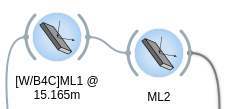
\includegraphics[width=0.8\textwidth]{images/DMM_oasys.png}
\caption{\label{fig:DMM_oasys} Double Multilayer Monochromator in Oasys Shadow.}
\end{figure}

\begin{figure}  % spans both columns
\begin{subfigure}{0.5\textwidth}
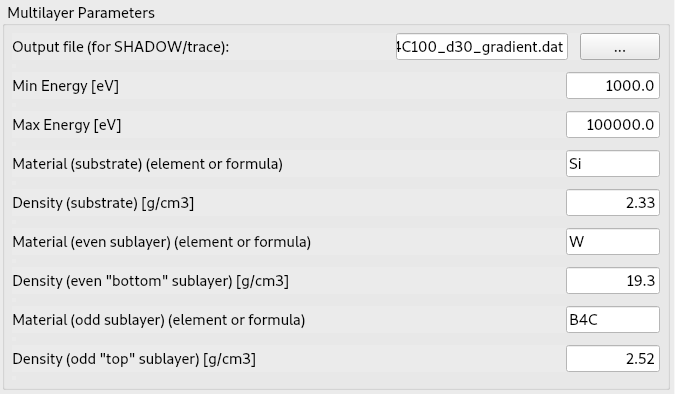
\includegraphics[width=\linewidth]{images/MLspecs_a.png}
\end{subfigure}
\hfill % maximize the horizontal distance between the graphs
\begin{subfigure}{0.5\textwidth}
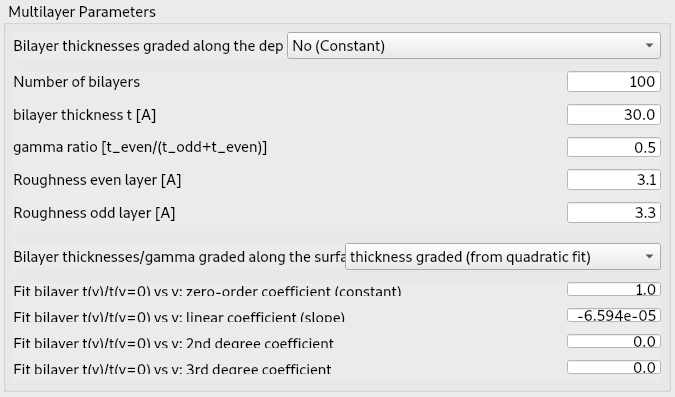
\includegraphics[width=\linewidth]{images/MLspecs_b.png}
\end{subfigure}
\caption{\label{fig:PreMLayer} PreMLayer widget settings in Shadow. }
\end{figure}

\begin{figure}  % spans both columns
\begin{subfigure}{0.33\textwidth}
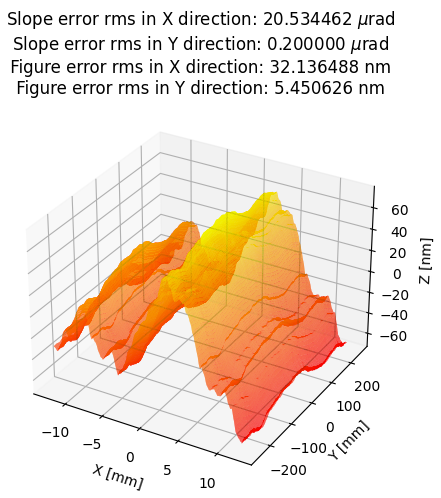
\includegraphics[width=0.9\linewidth]{./../figures/slope_error/surface_error_profile_500x25_02x20urad.png}
\end{subfigure}
\hfill % maximize the horizontal distance between the graphs
\begin{subfigure}{0.33\textwidth}
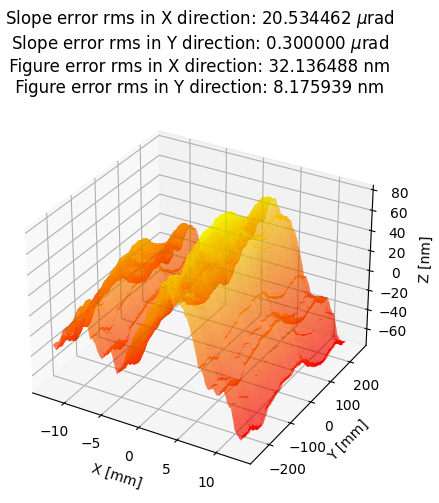
\includegraphics[width=0.9\linewidth]{./../figures/slope_error/surface_error_profile_500x25_03x20urad.png}
\end{subfigure}
\hfill % maximize the horizontal distance between the graphs
\begin{subfigure}{0.33\textwidth}
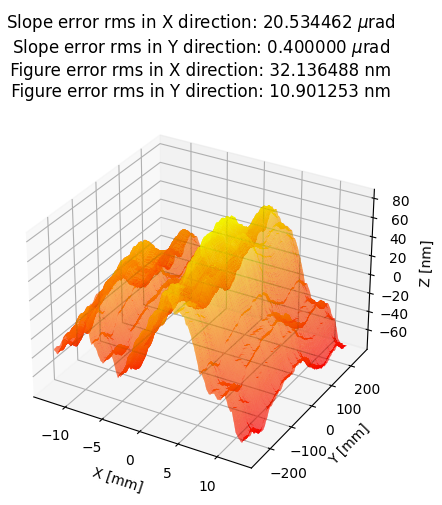
\includegraphics[width=0.9\linewidth]{./../figures/slope_error/surface_error_profile_500x25_04x20urad.png}
\end{subfigure}
\caption{\label{fig:fractals} Modified mirror surfaces. }
\end{figure}

%%%%%%%%%%%%%%%%%%%%%%%%%%%%%%%%%%%%%%%%%%%%%%%%%%%%%%%%%%%%%%%%%%%%%%%%%%%%%%%%%%
\clearpage
\subsubsection{0.1 urad}
\begin{figure}[H]
\centering
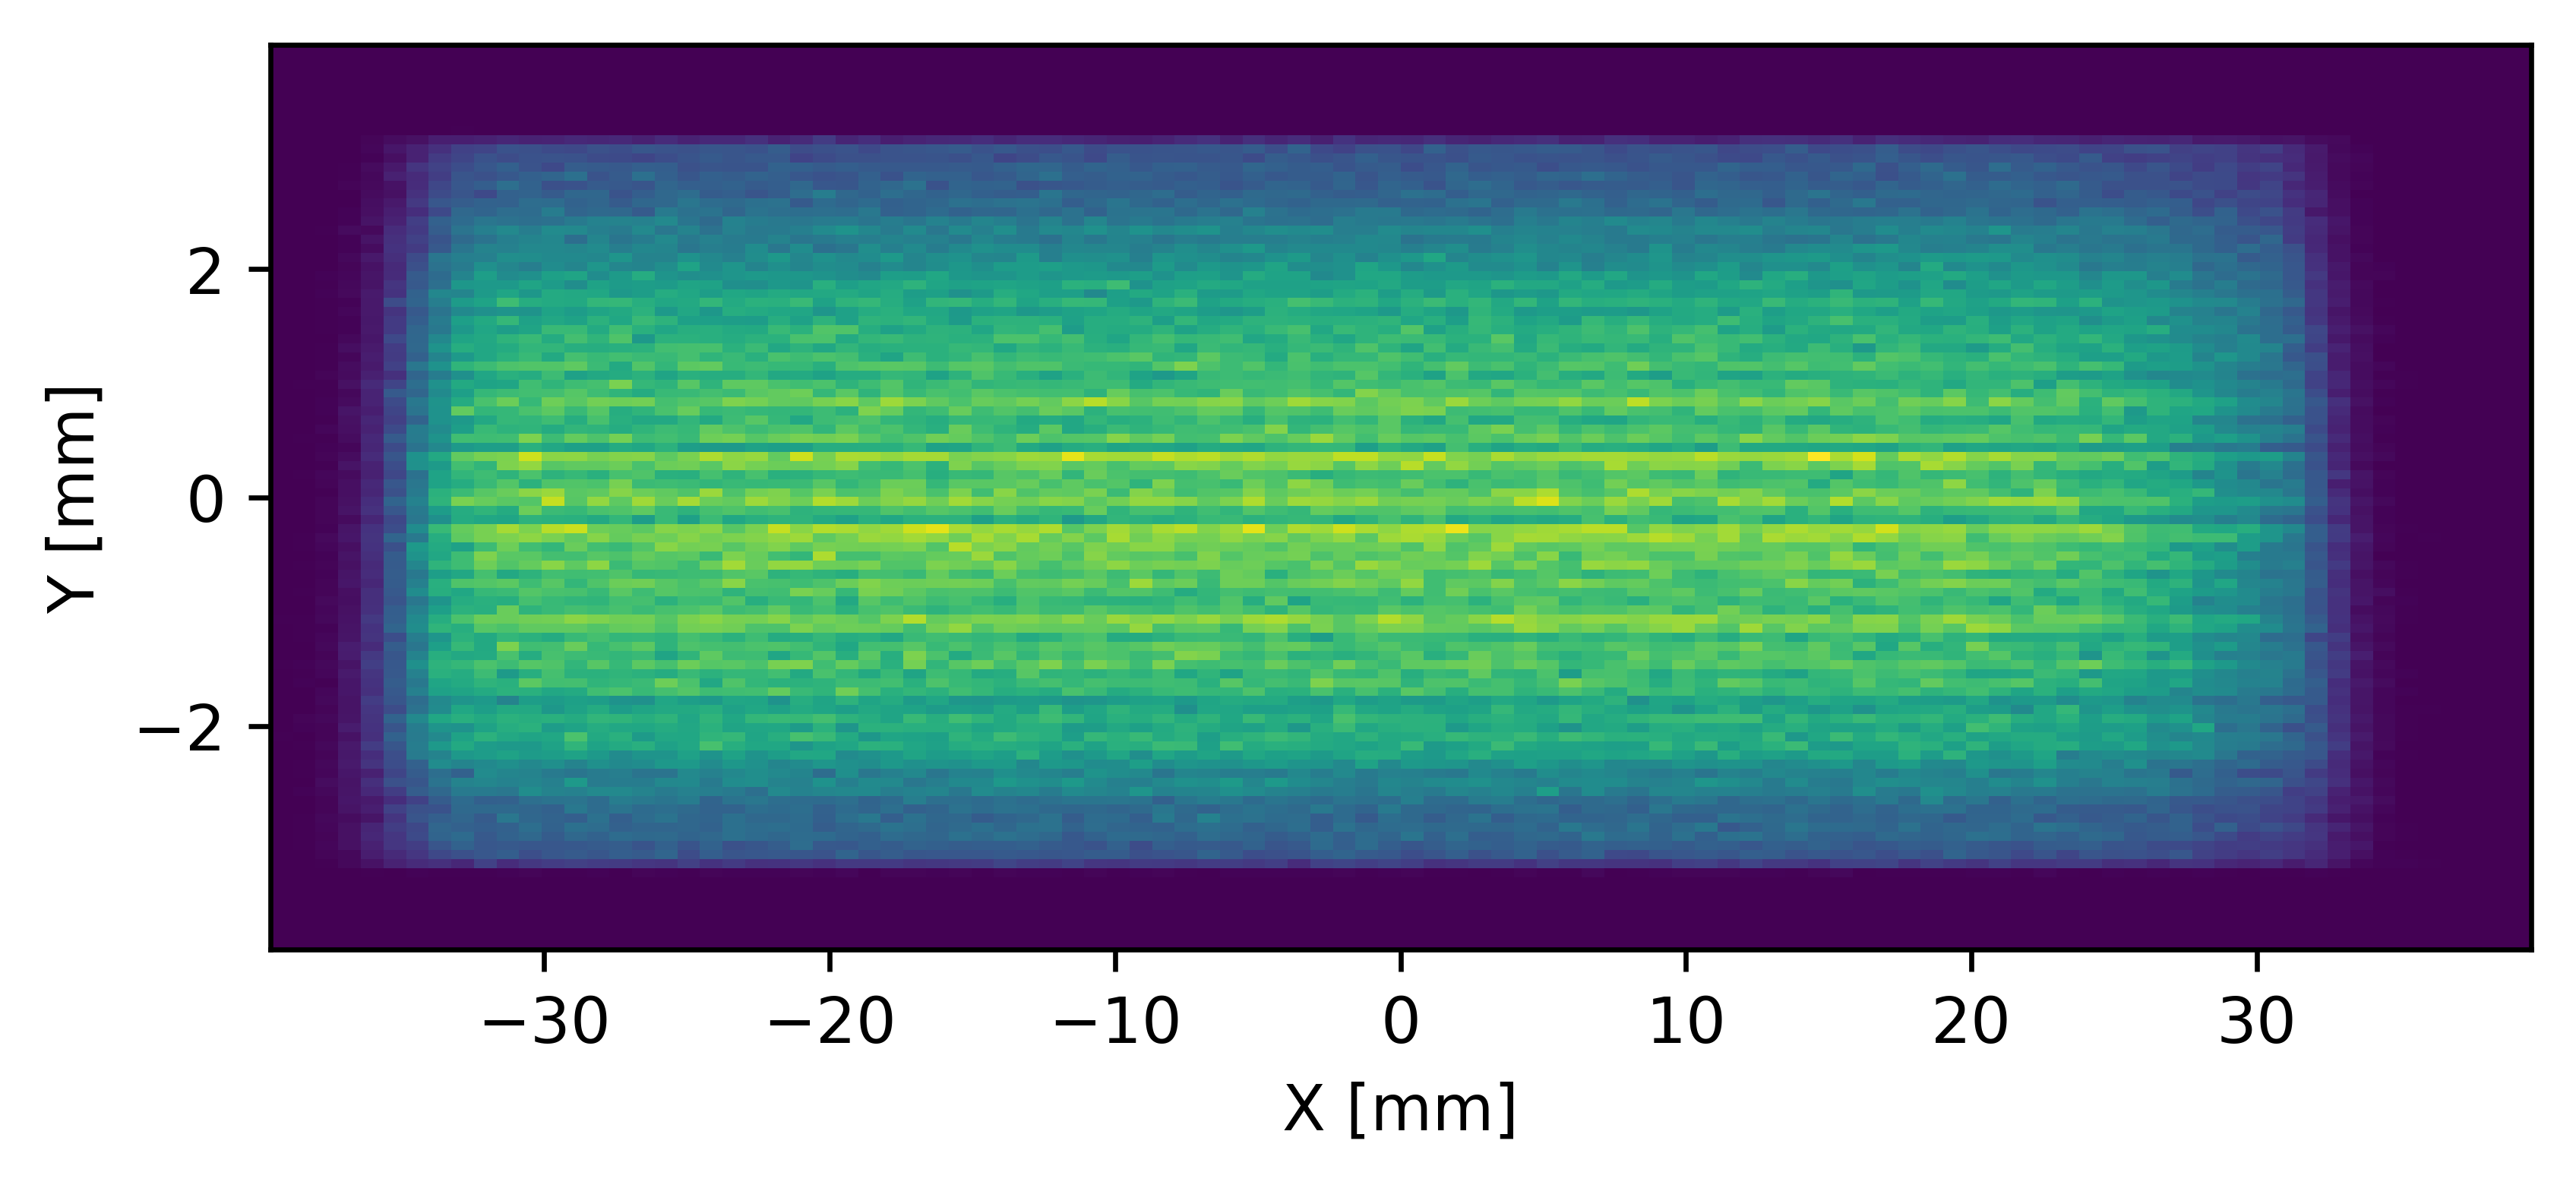
\includegraphics[width=0.9\linewidth]{./../figures/slope_error/WB4C_d30_d-spacing_gradient_45keV_slope_error01urad.png}
\end{figure}

\begin{figure}[H]
\centering
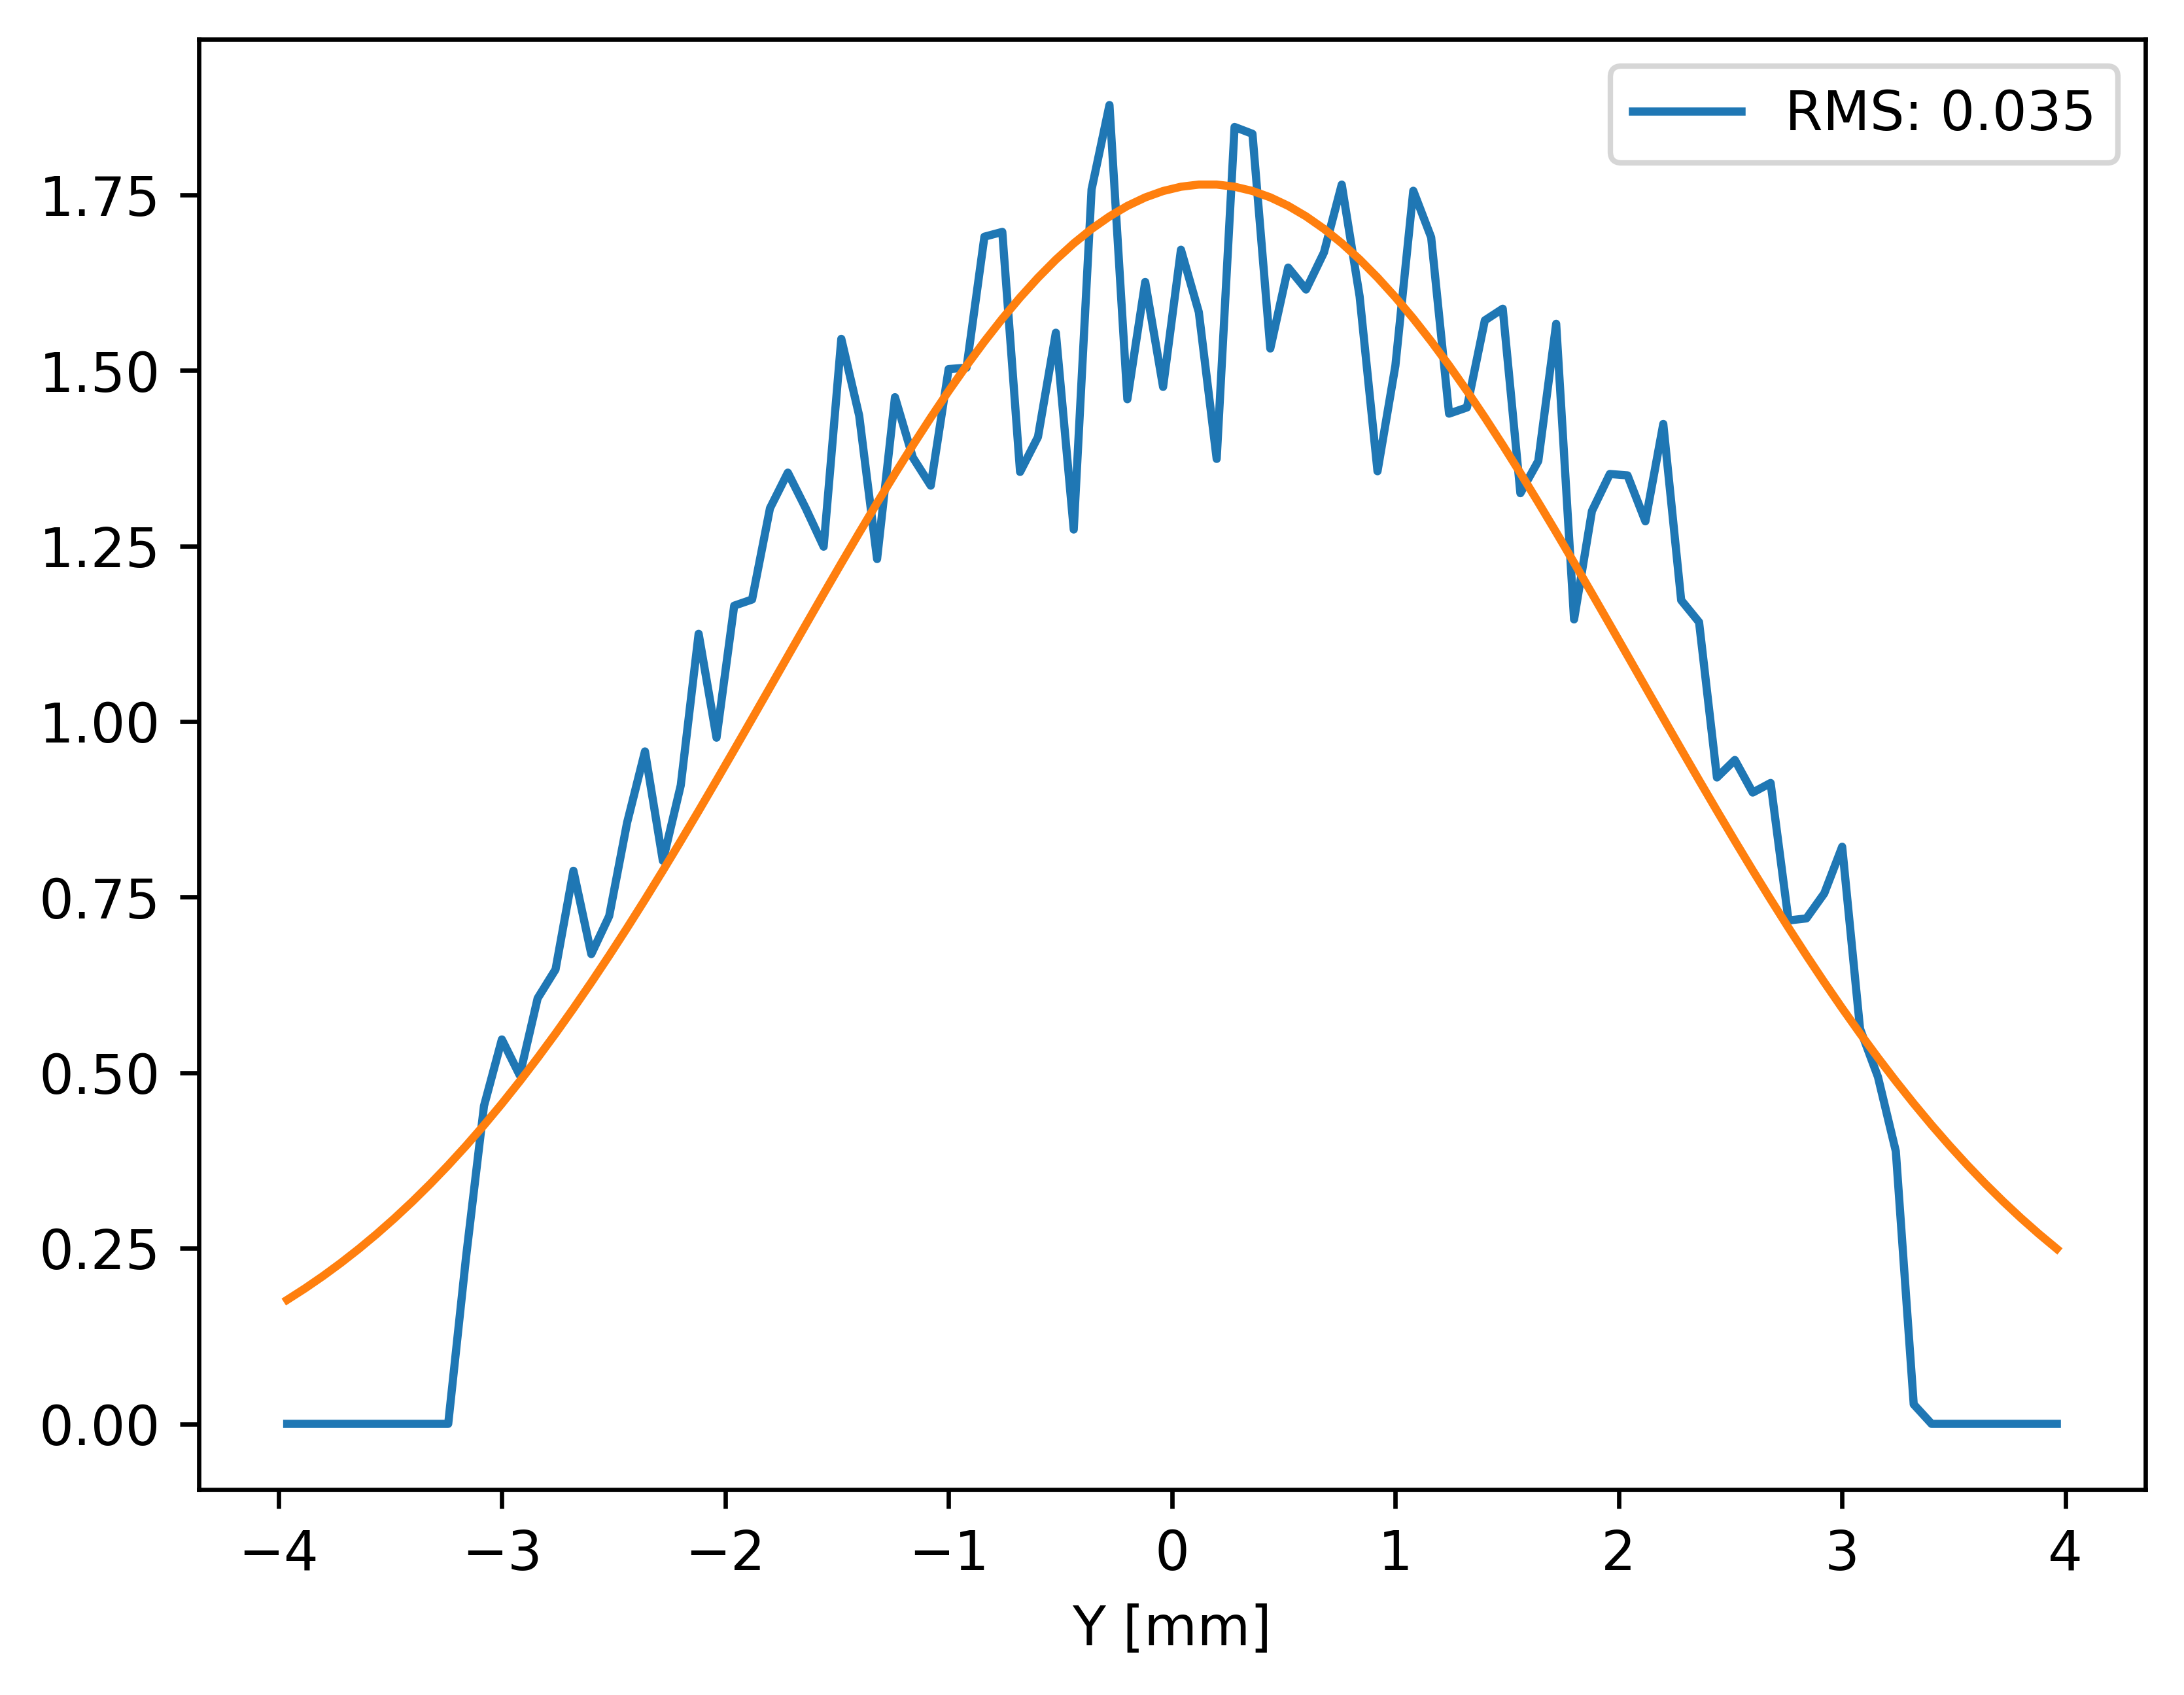
\includegraphics[width=0.9\linewidth]{./../figures/slope_error/WB4C_d30_d-spacing_gradient_45keV_slope_error01urad_Yprofile.png}
\caption{0.1 urad}
\label{fig:01urad}
\end{figure}

\clearpage
\subsubsection{0.2 urad}
\begin{figure}[H]
\centering
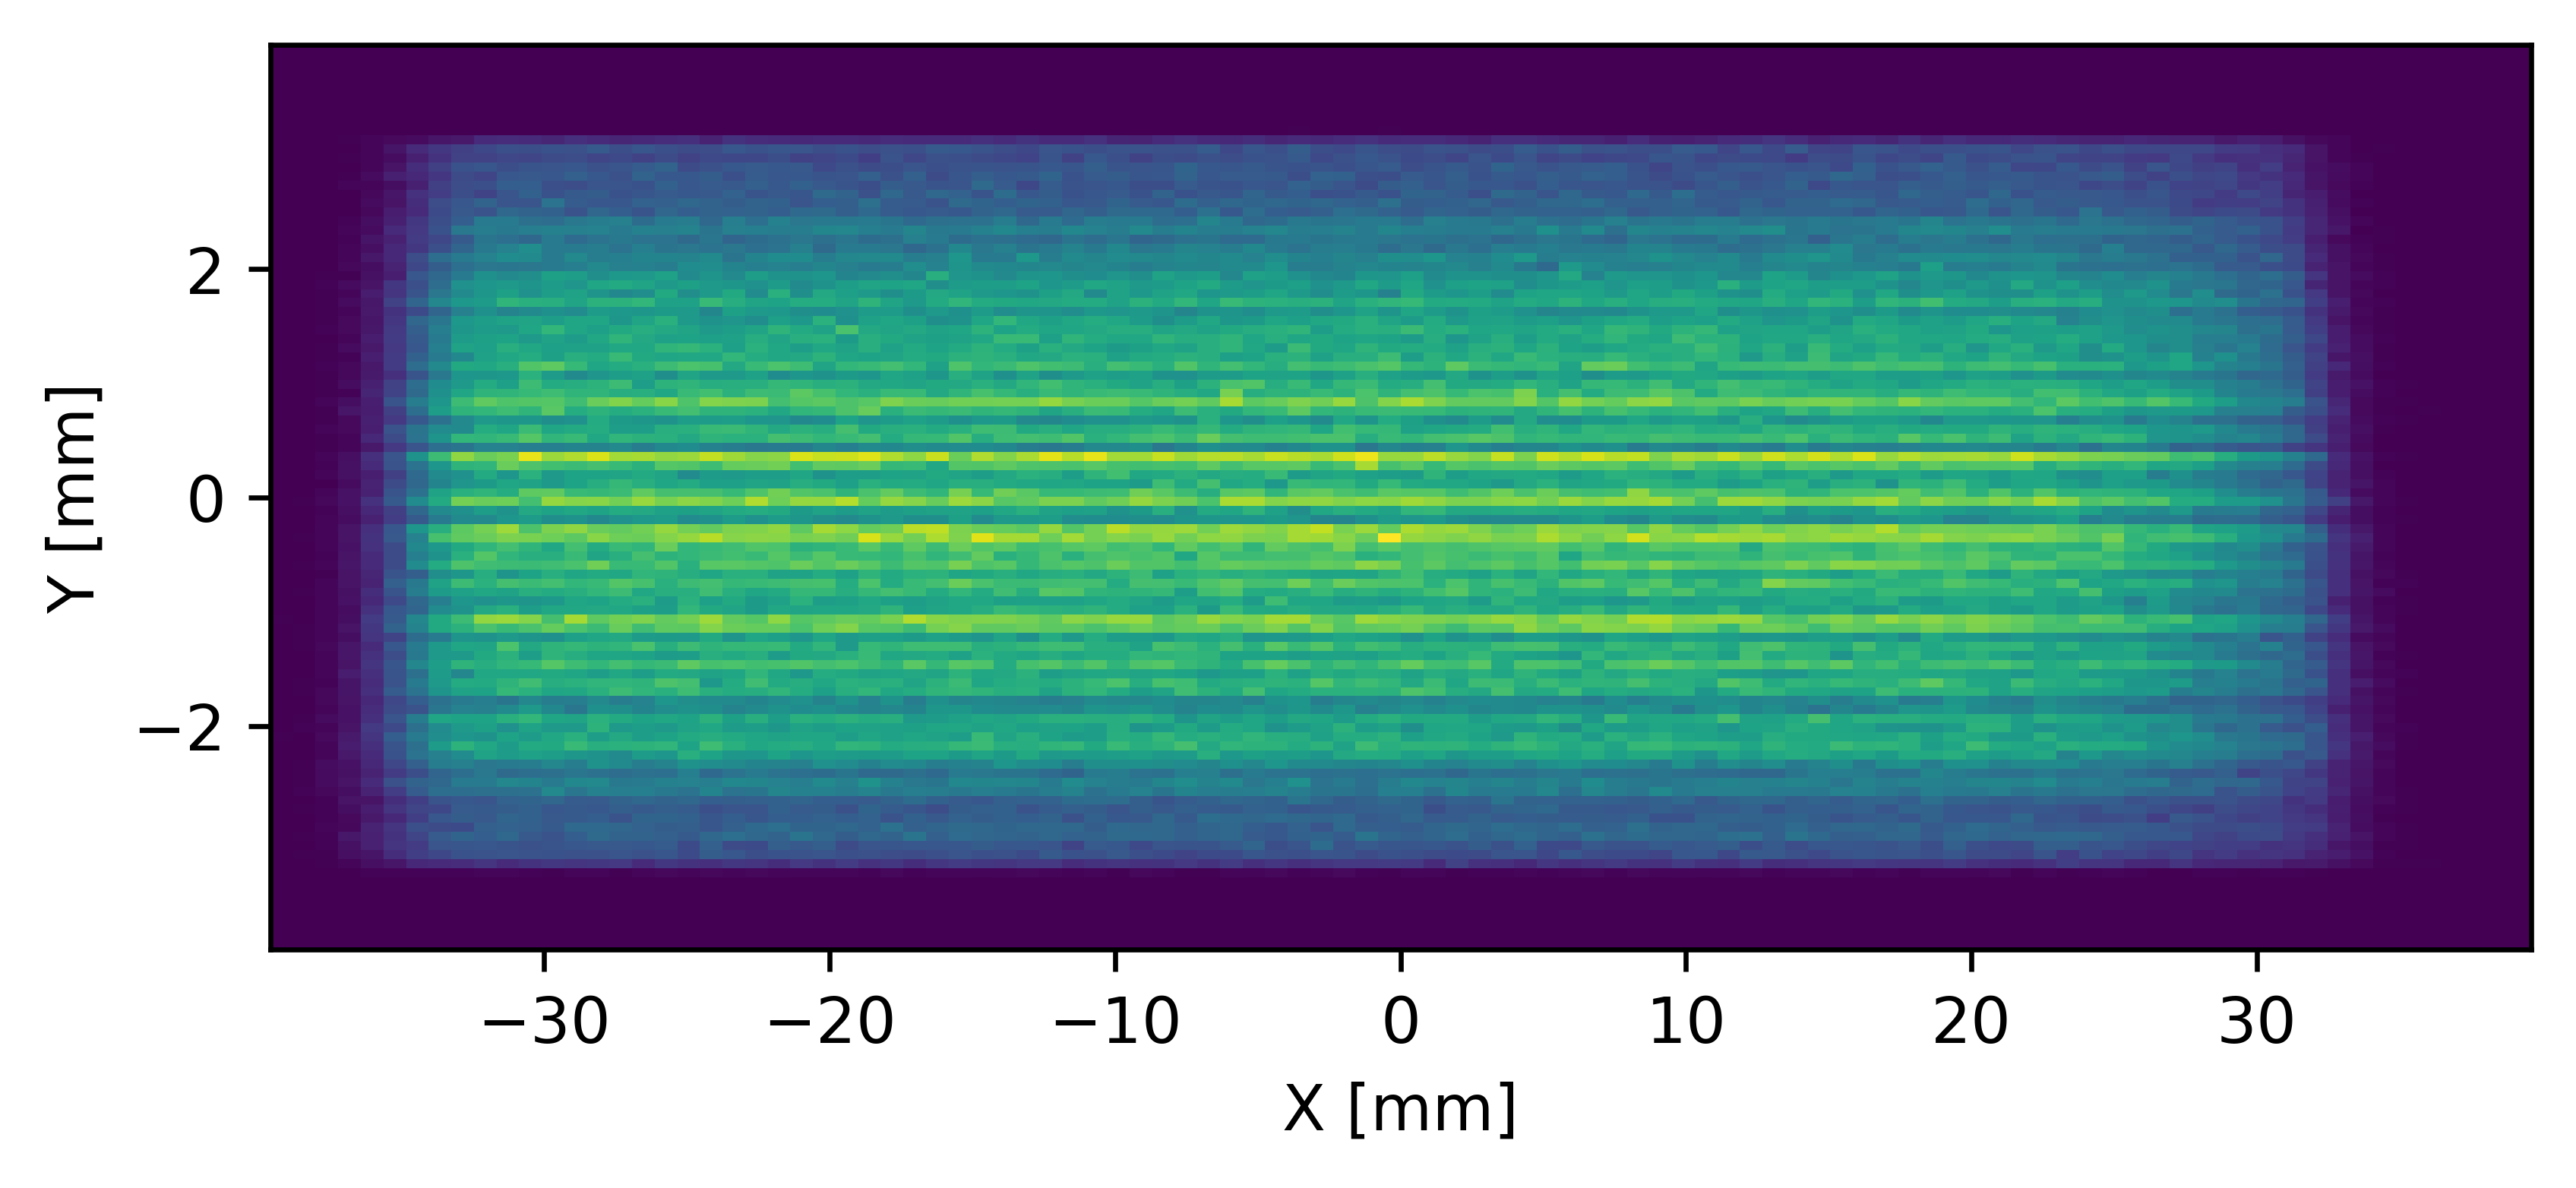
\includegraphics[width=0.9\linewidth]{./../figures/slope_error/WB4C_d30_d-spacing_gradient_45keV_slope_error02urad.png}
\end{figure}

\begin{figure}[H]
\centering
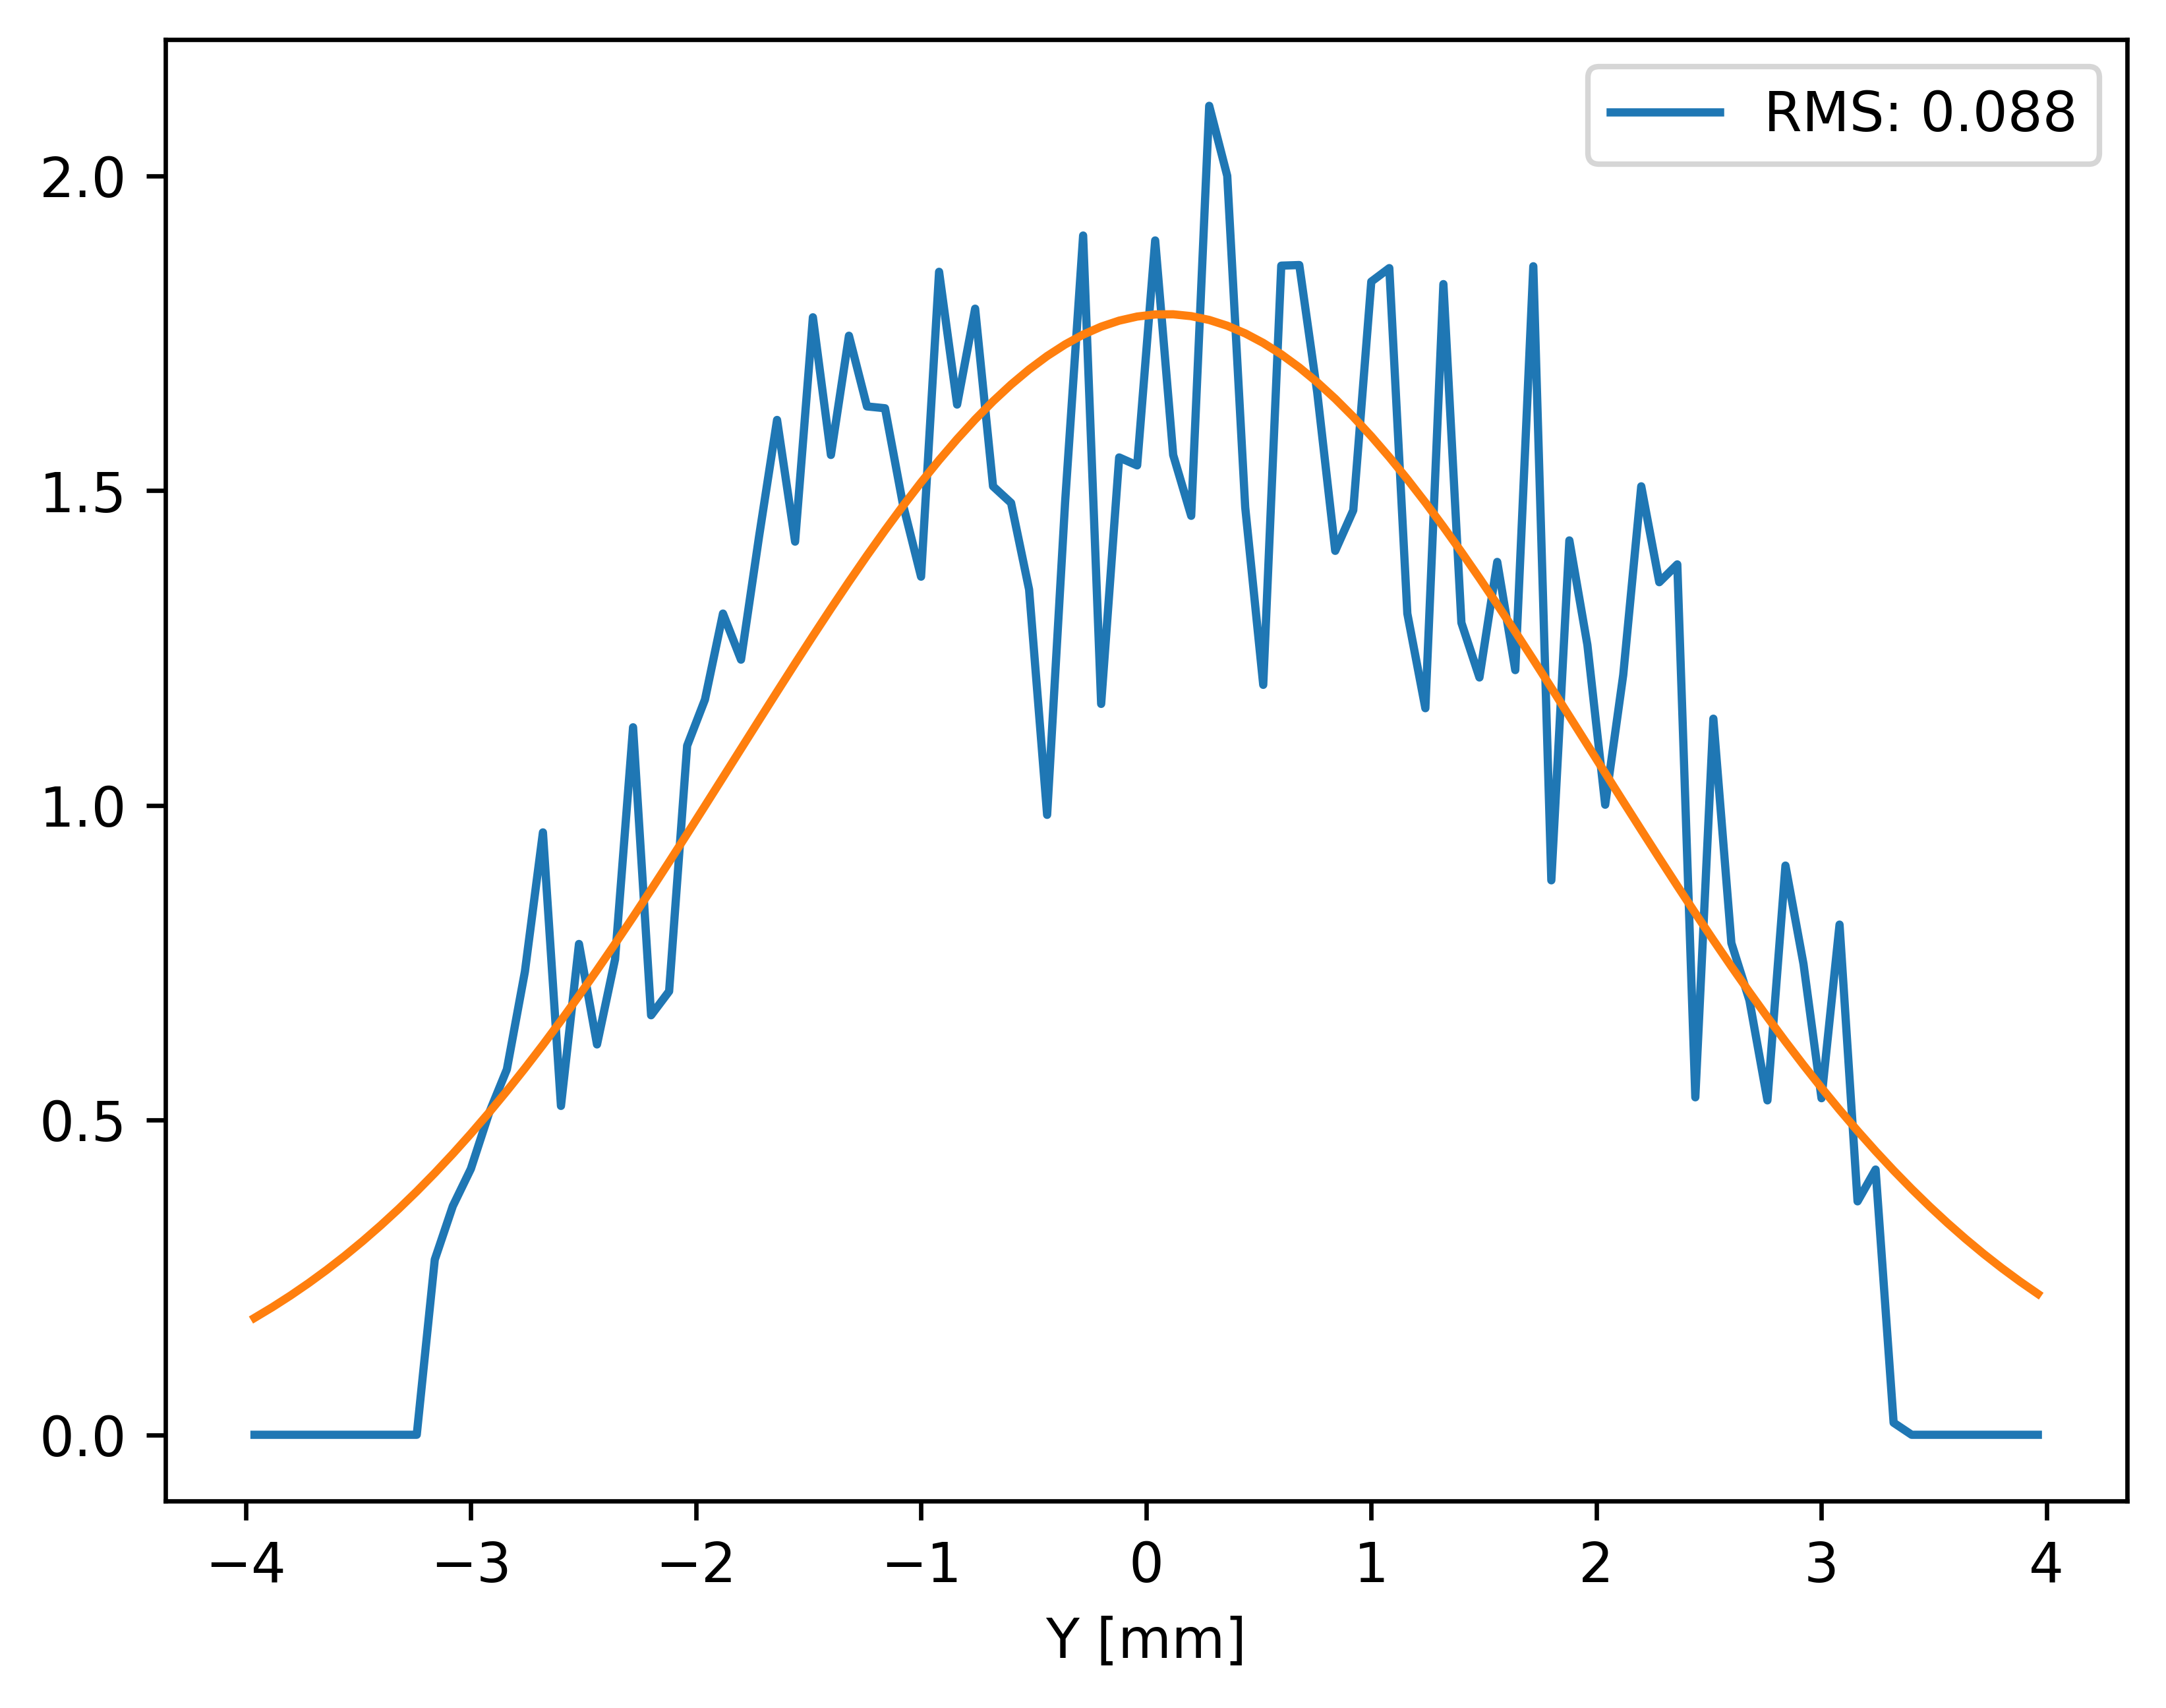
\includegraphics[width=0.9\linewidth]{./../figures/slope_error/WB4C_d30_d-spacing_gradient_45keV_slope_error02urad_Yprofile.png}
\caption{0.2 urad}
\label{fig:02urad}
\end{figure}

\clearpage
\subsubsection{0.3 urad}
\begin{figure}[H]
\centering
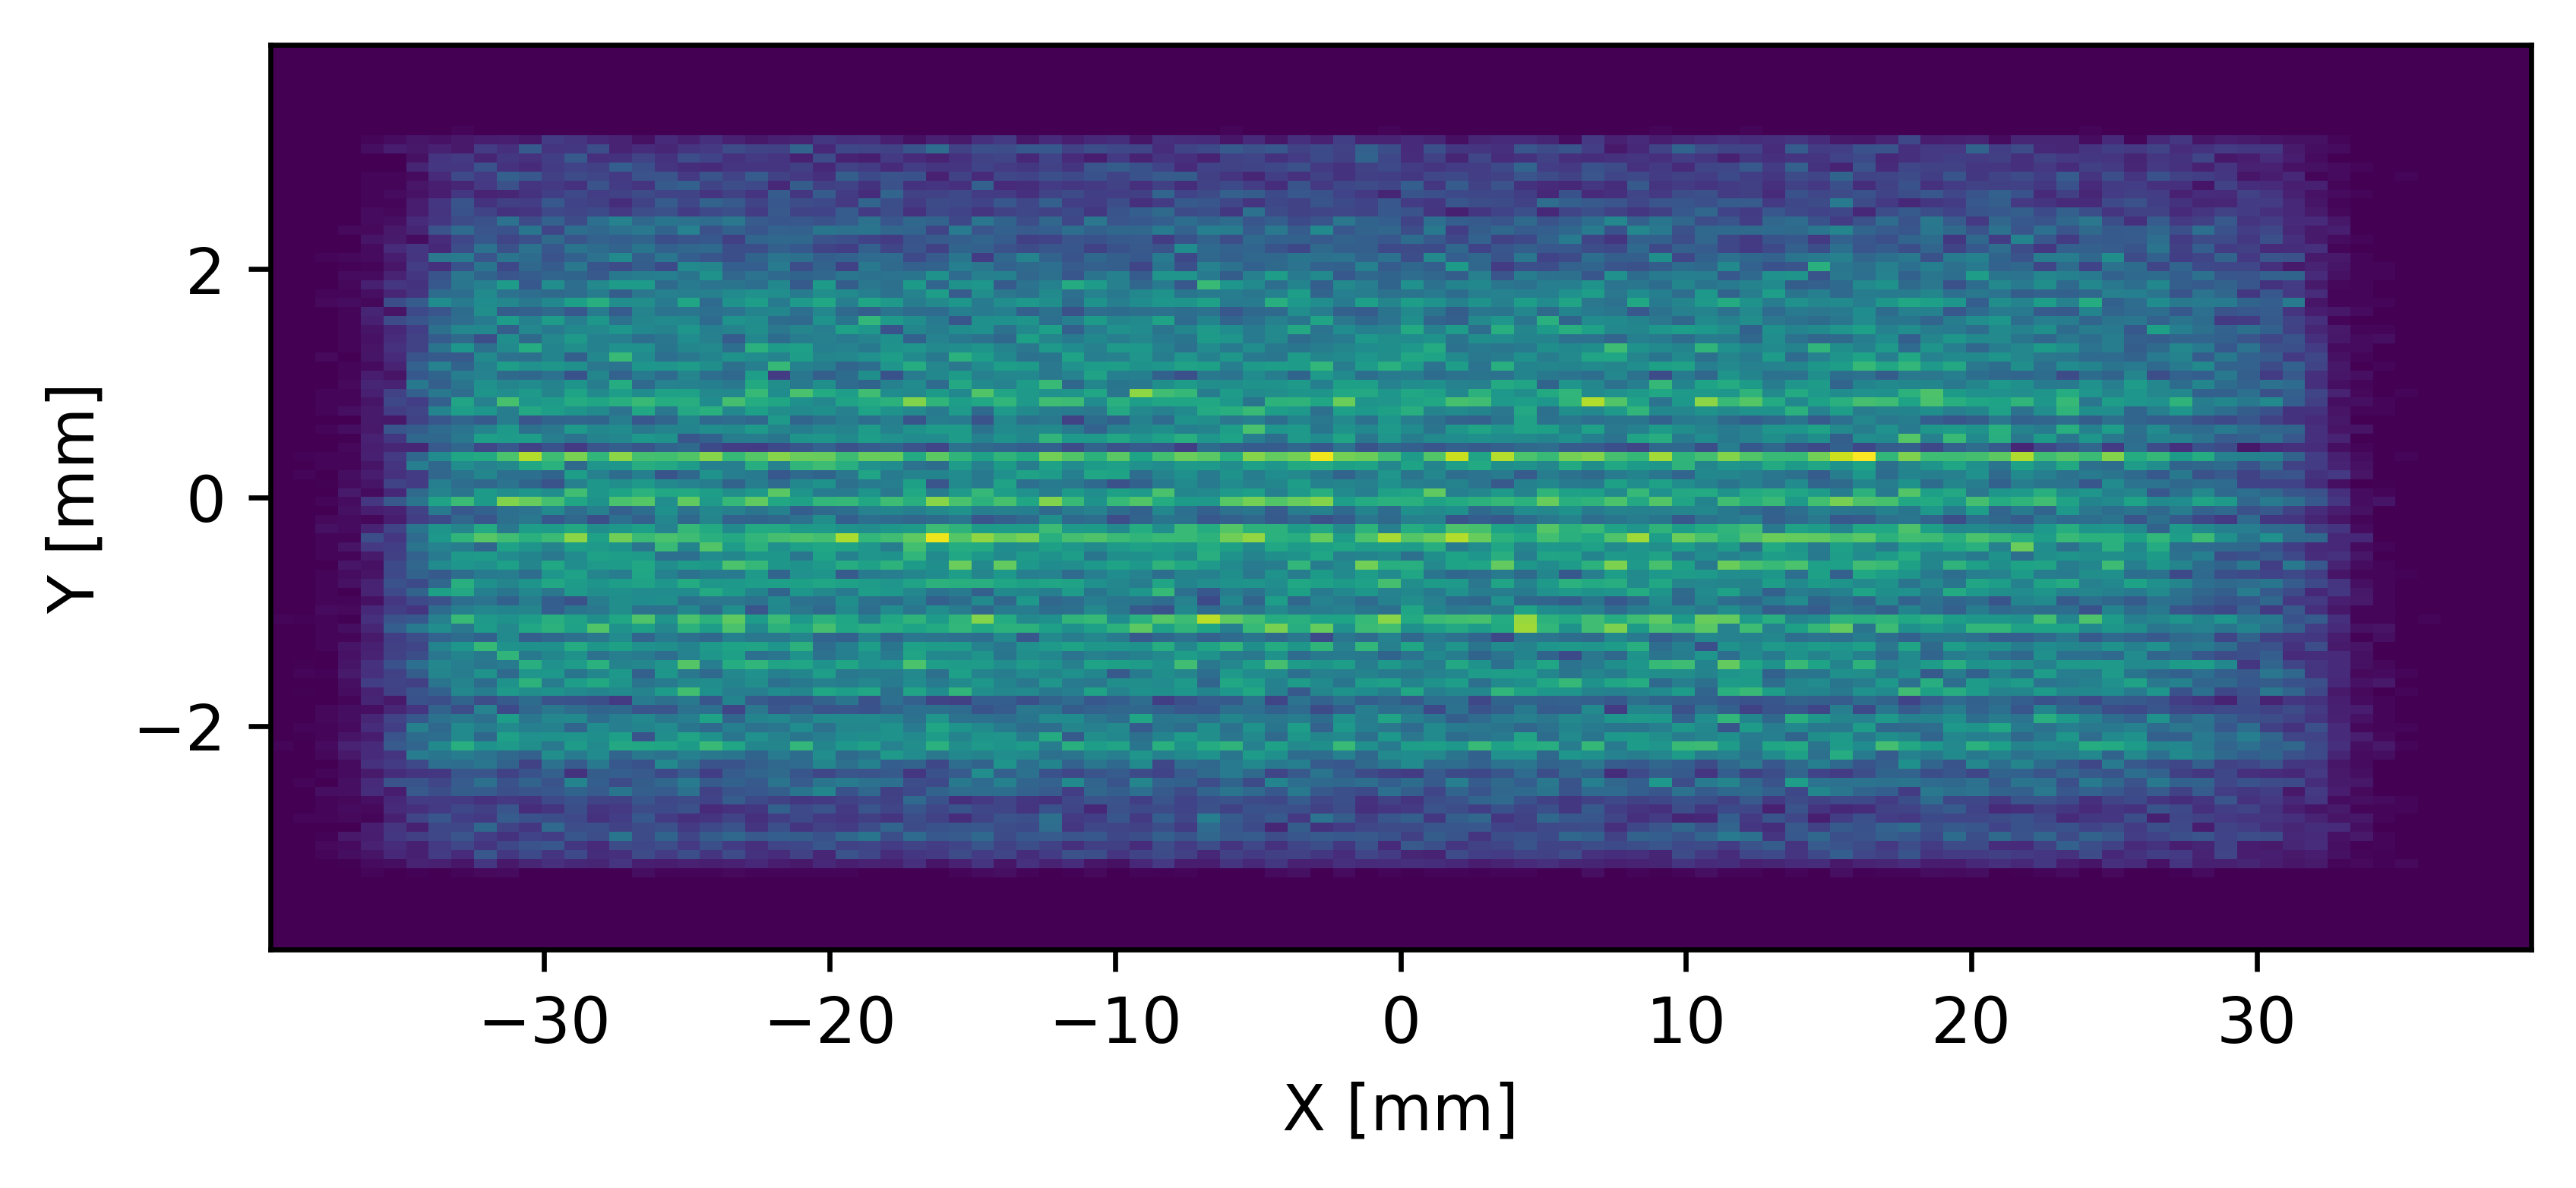
\includegraphics[width=0.9\linewidth]{./../figures/slope_error/WB4C_d30_d-spacing_gradient_45keV_slope_error03urad.png}
\end{figure}

\begin{figure}[H]
\centering
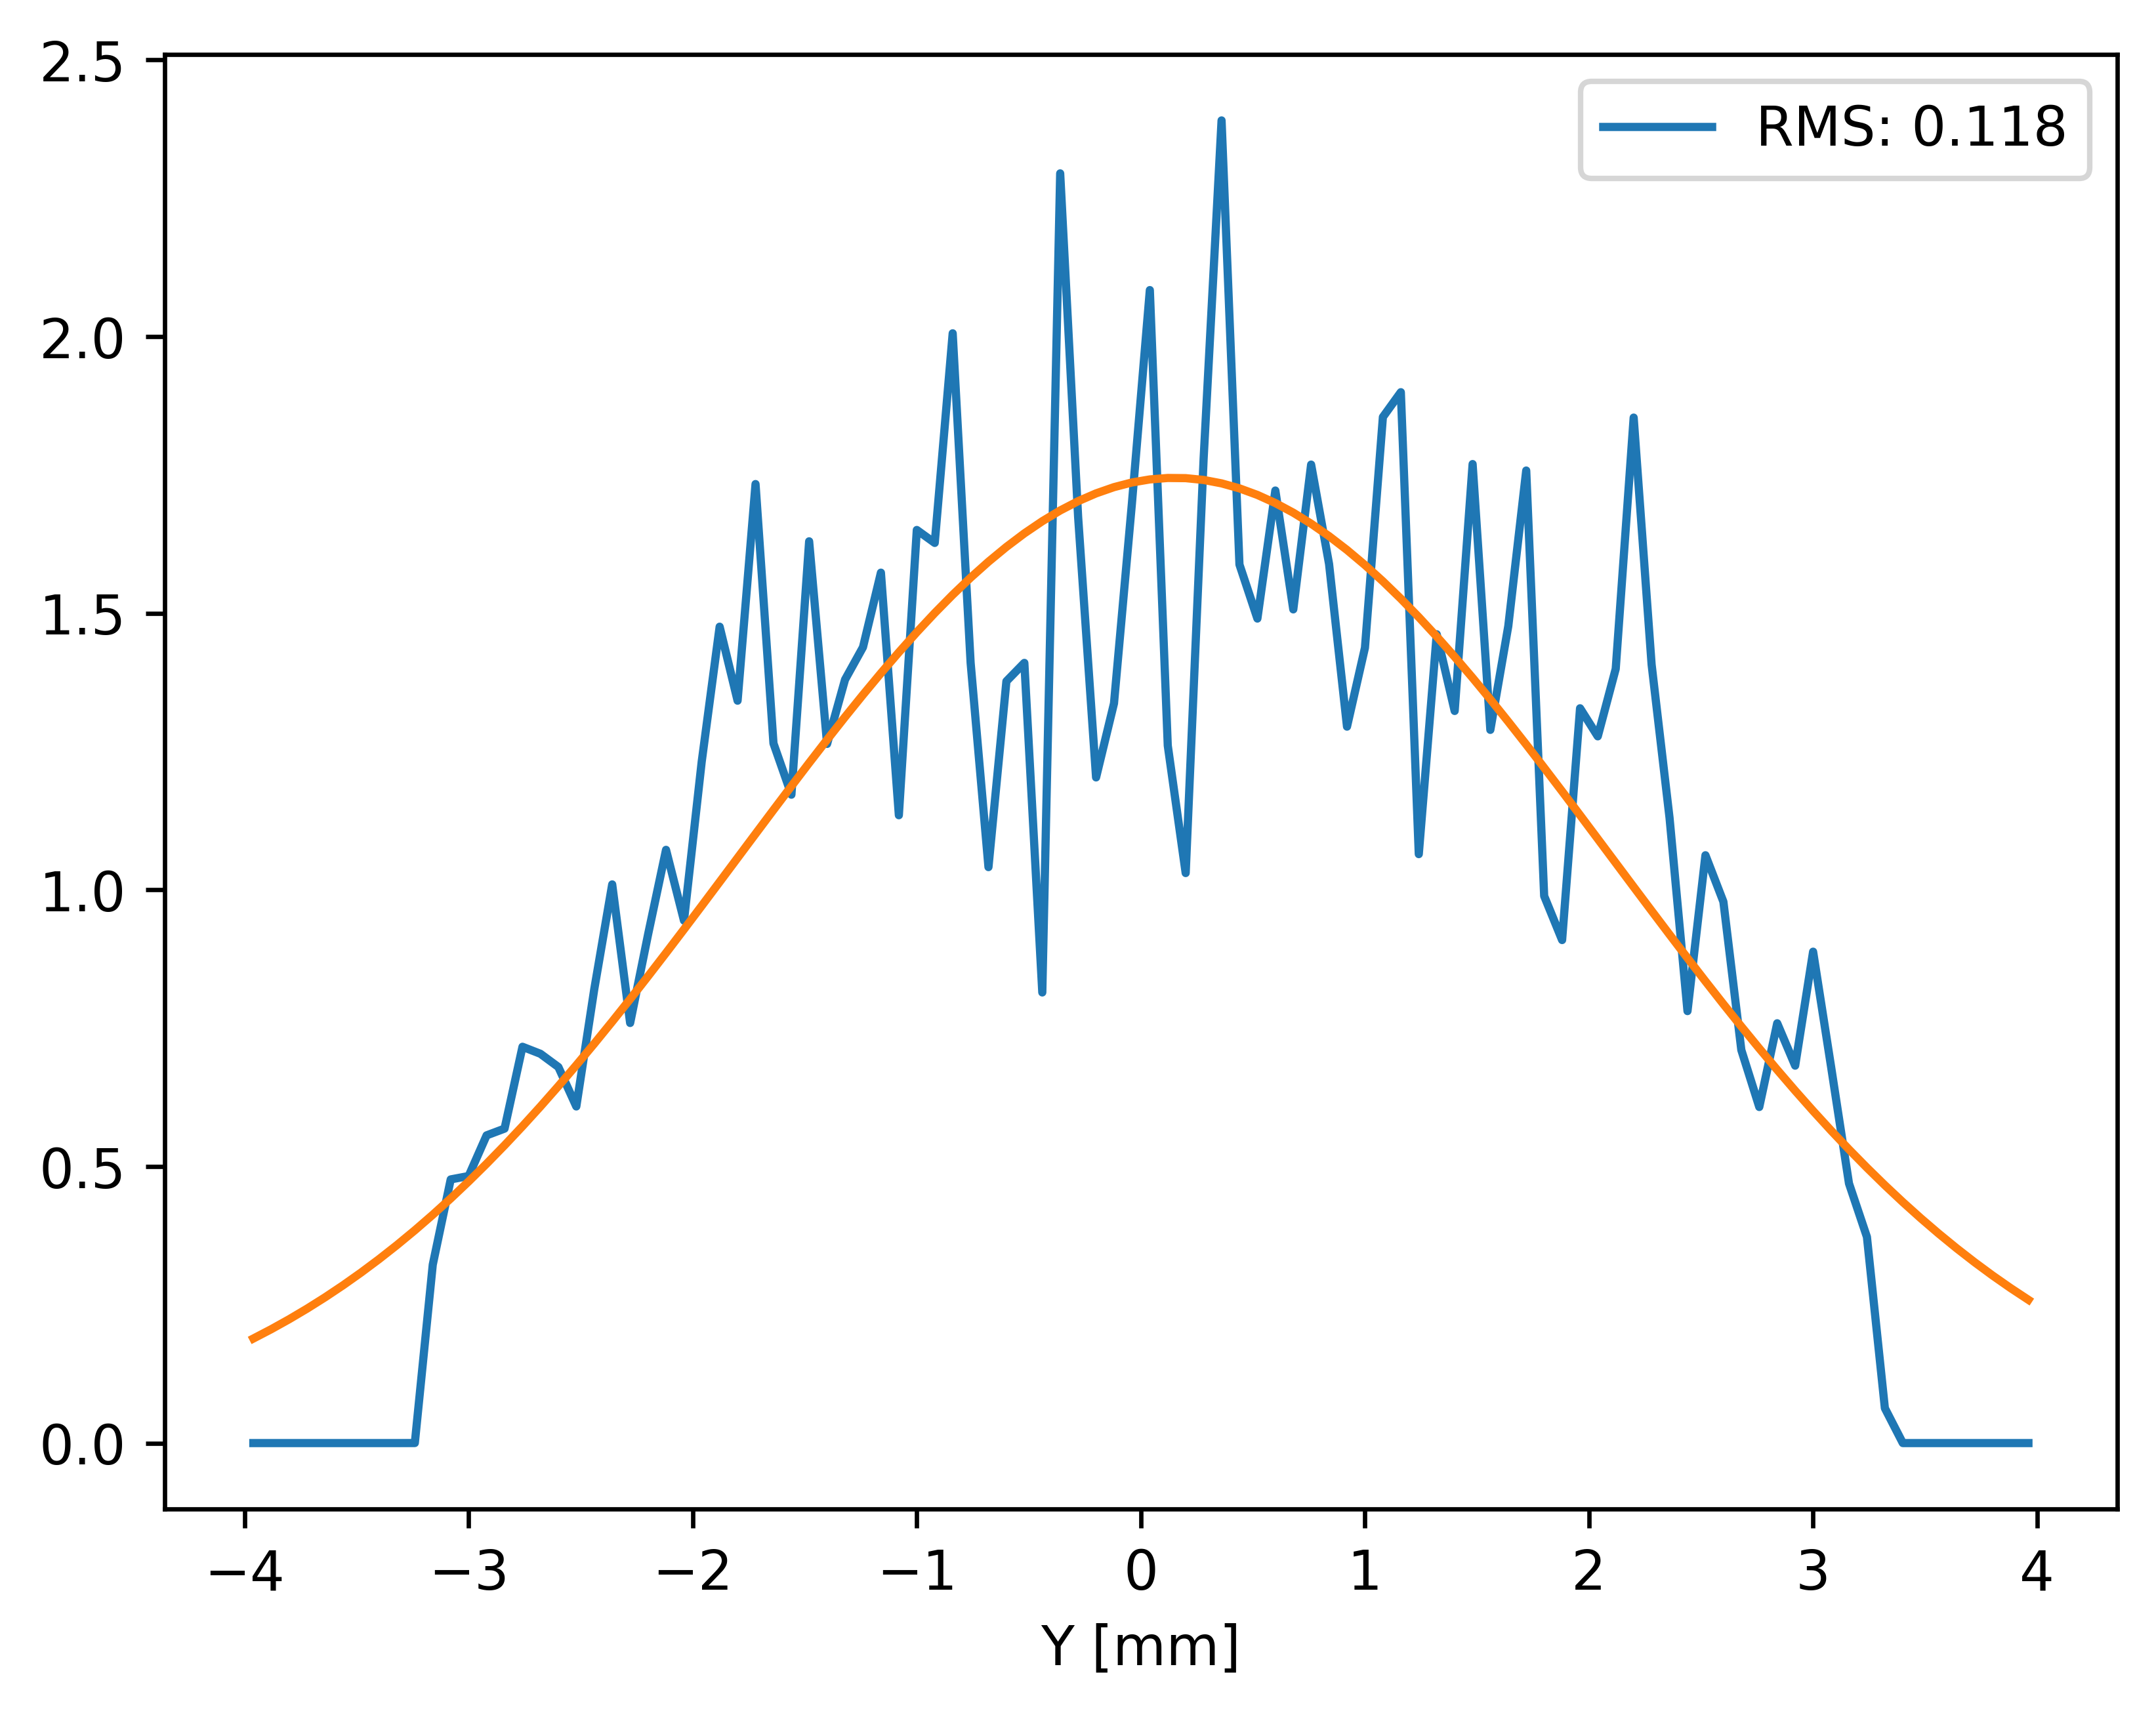
\includegraphics[width=0.9\linewidth]{./../figures/slope_error/WB4C_d30_d-spacing_gradient_45keV_slope_error03urad_Yprofile.png}
\caption{0.3 urad}
\label{fig:03urad}
\end{figure}

\clearpage
\subsubsection{0.4 urad}
\begin{figure}[H]
\centering
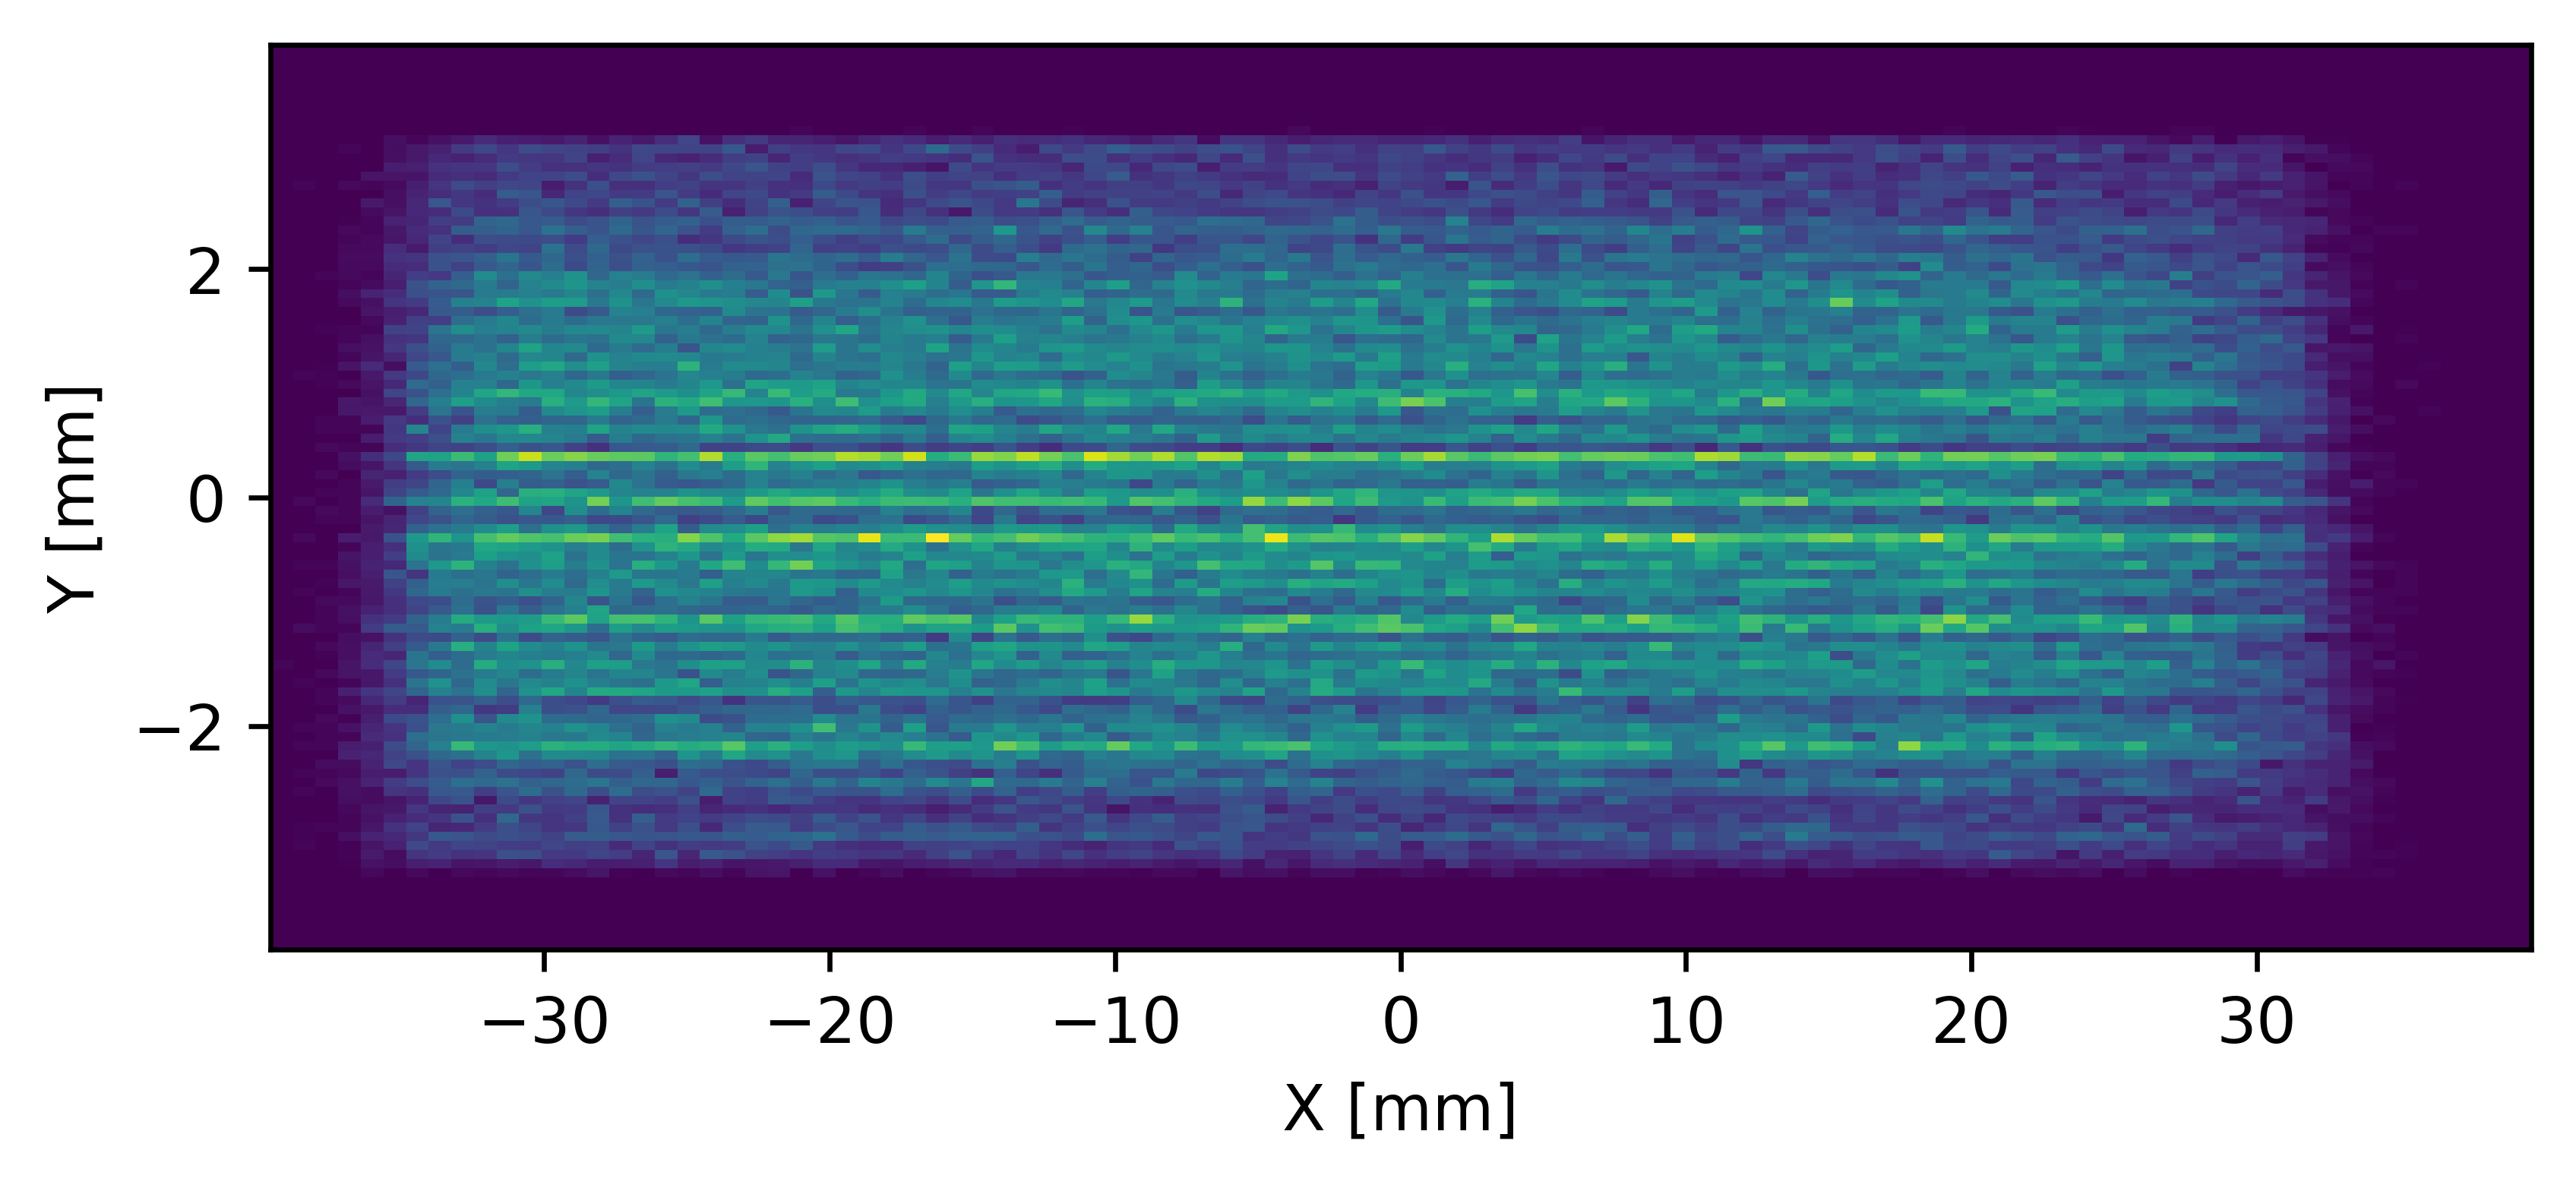
\includegraphics[width=0.9\linewidth]{./../figures/slope_error/WB4C_d30_d-spacing_gradient_45keV_slope_error04urad.png}
\end{figure}

\begin{figure}[H]
\centering
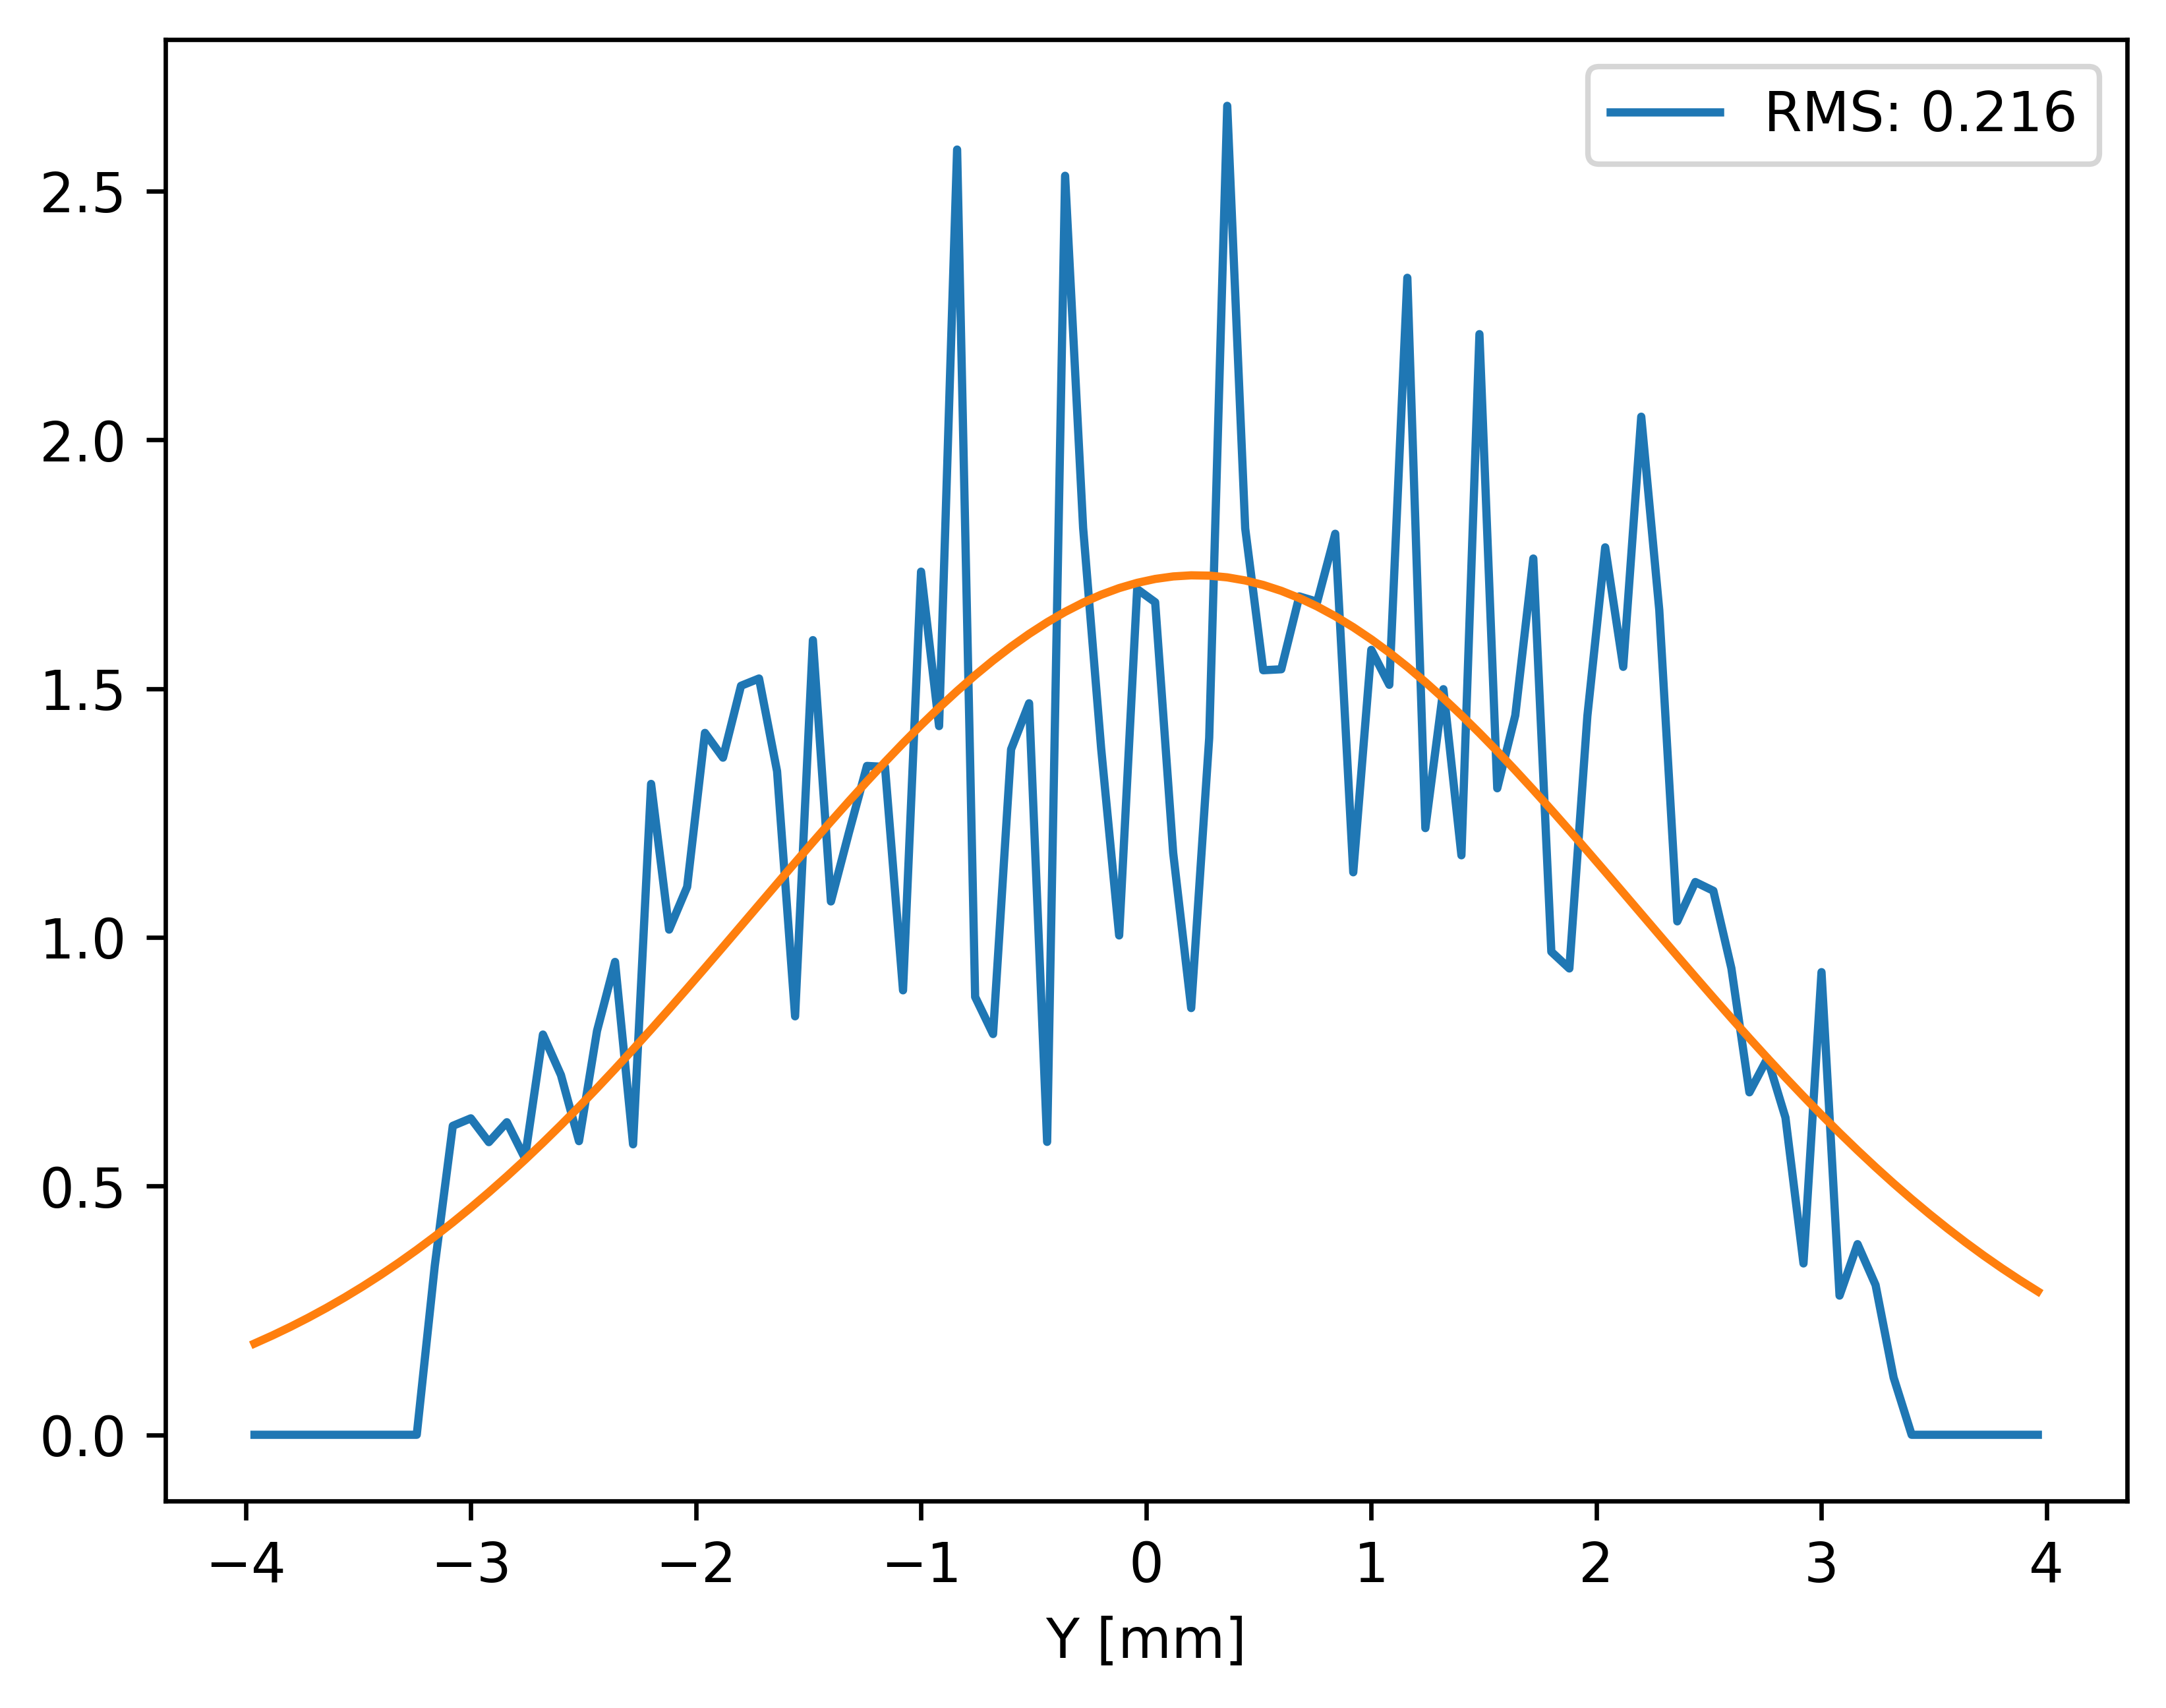
\includegraphics[width=0.9\linewidth]{./../figures/slope_error/WB4C_d30_d-spacing_gradient_45keV_slope_error04urad_Yprofile.png}
\caption{0.4 urad}
\label{fig:04urad}
\end{figure}

\clearpage
\subsubsection{0.5 urad}
\begin{figure}[H]
\centering
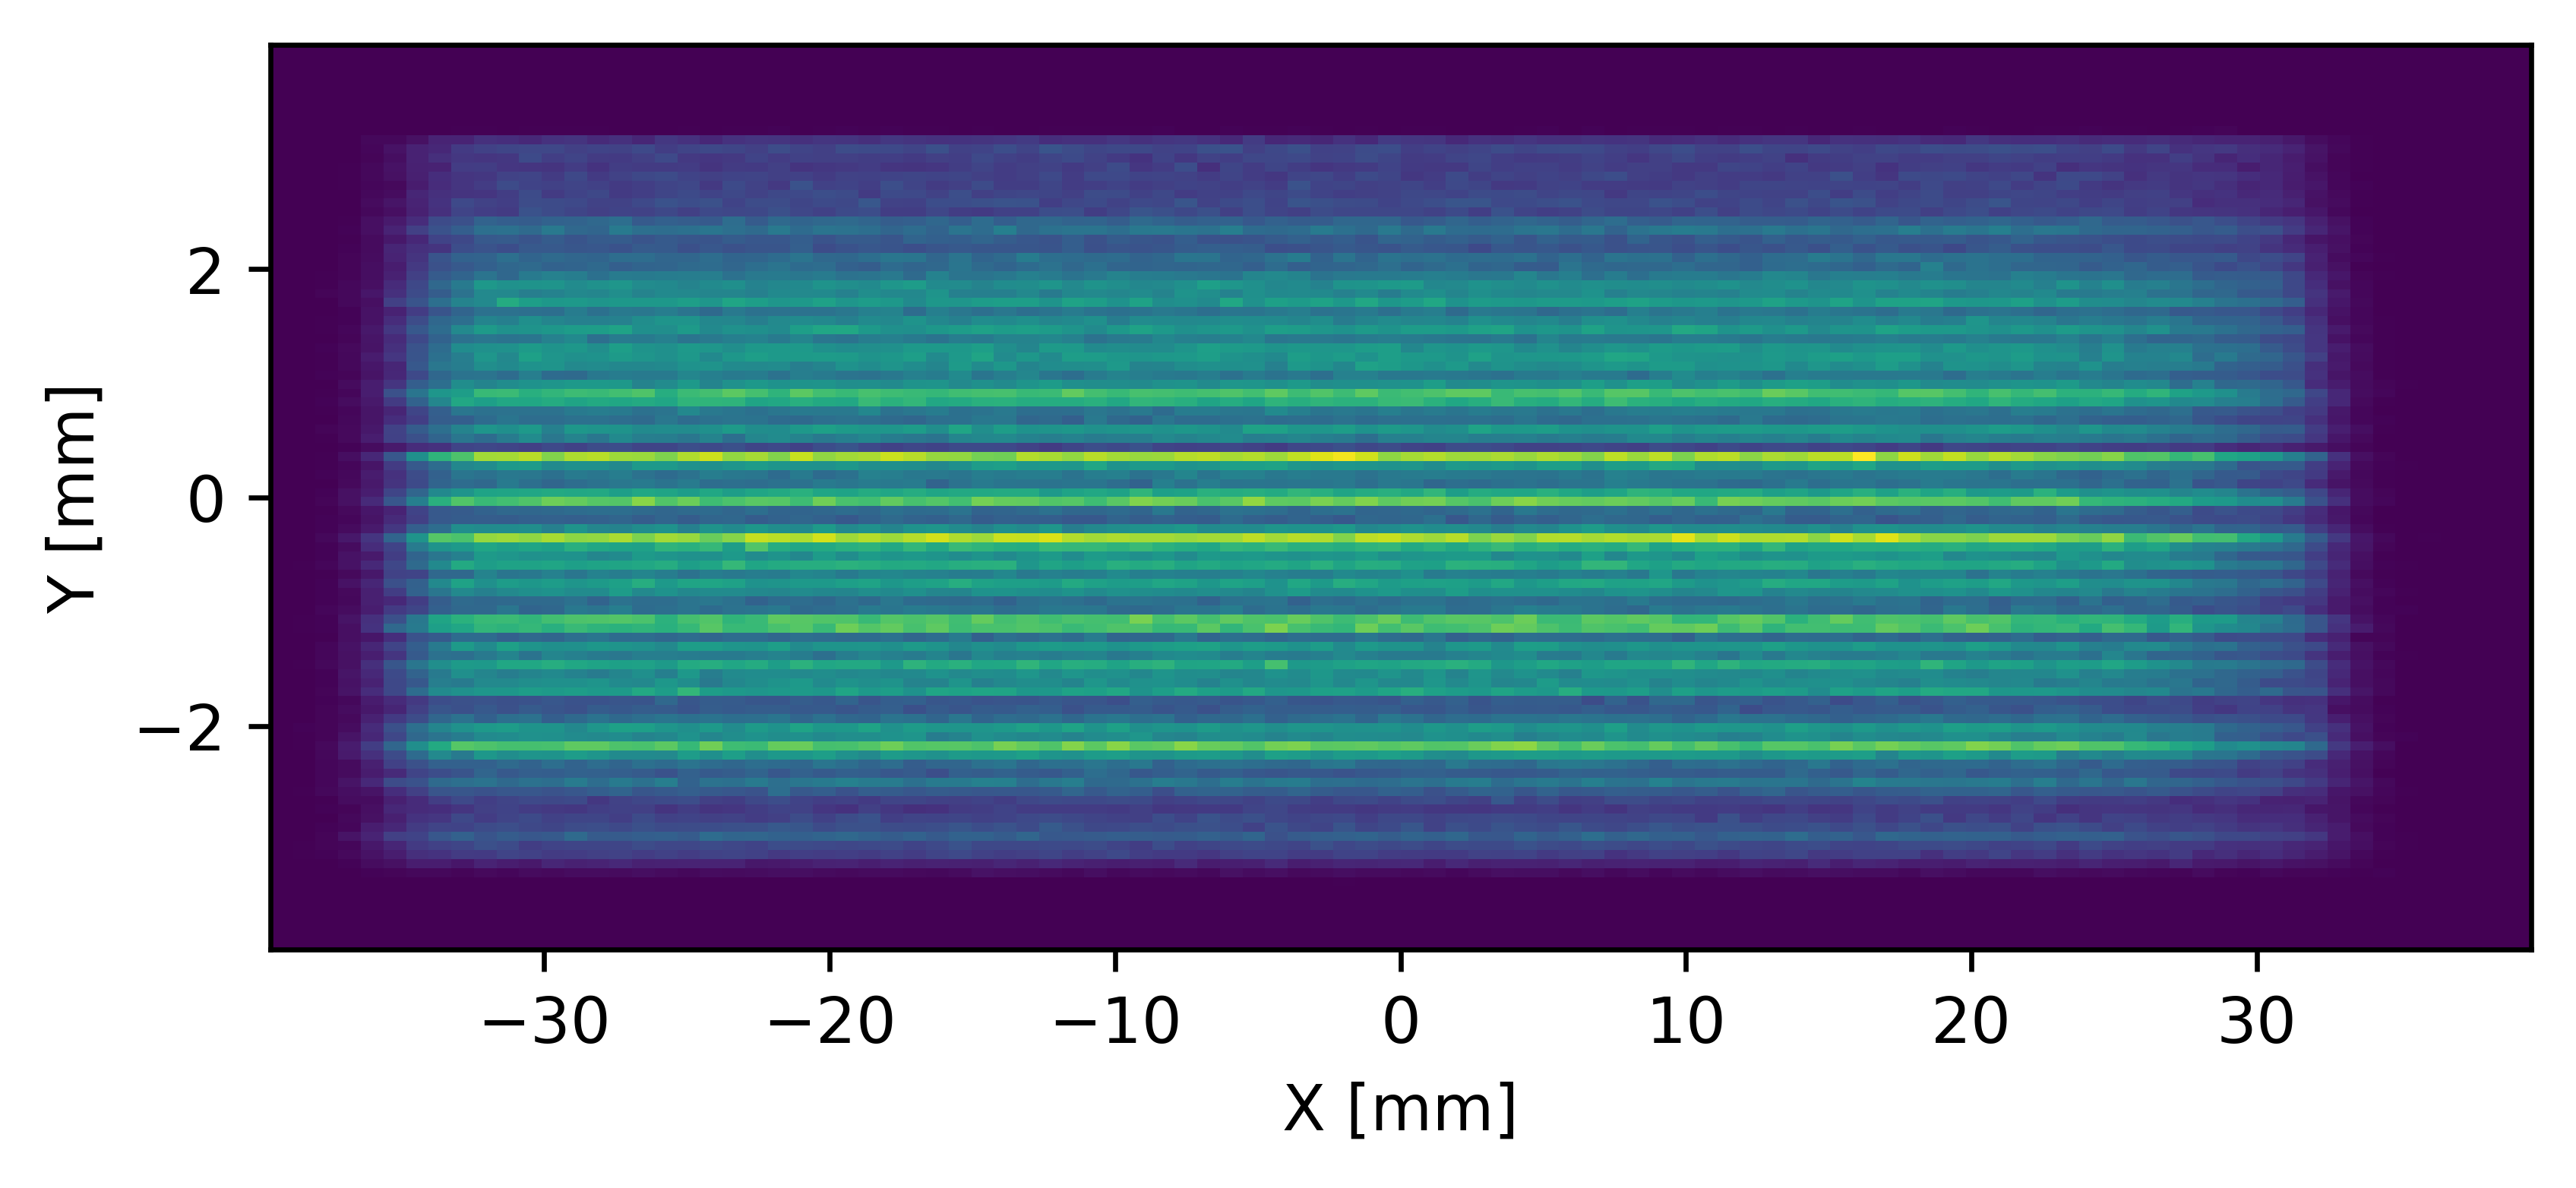
\includegraphics[width=0.9\linewidth]{./../figures/slope_error/WB4C_d30_d-spacing_gradient_45keV_slope_error05urad.png}
\end{figure}

\begin{figure}[H]
\centering
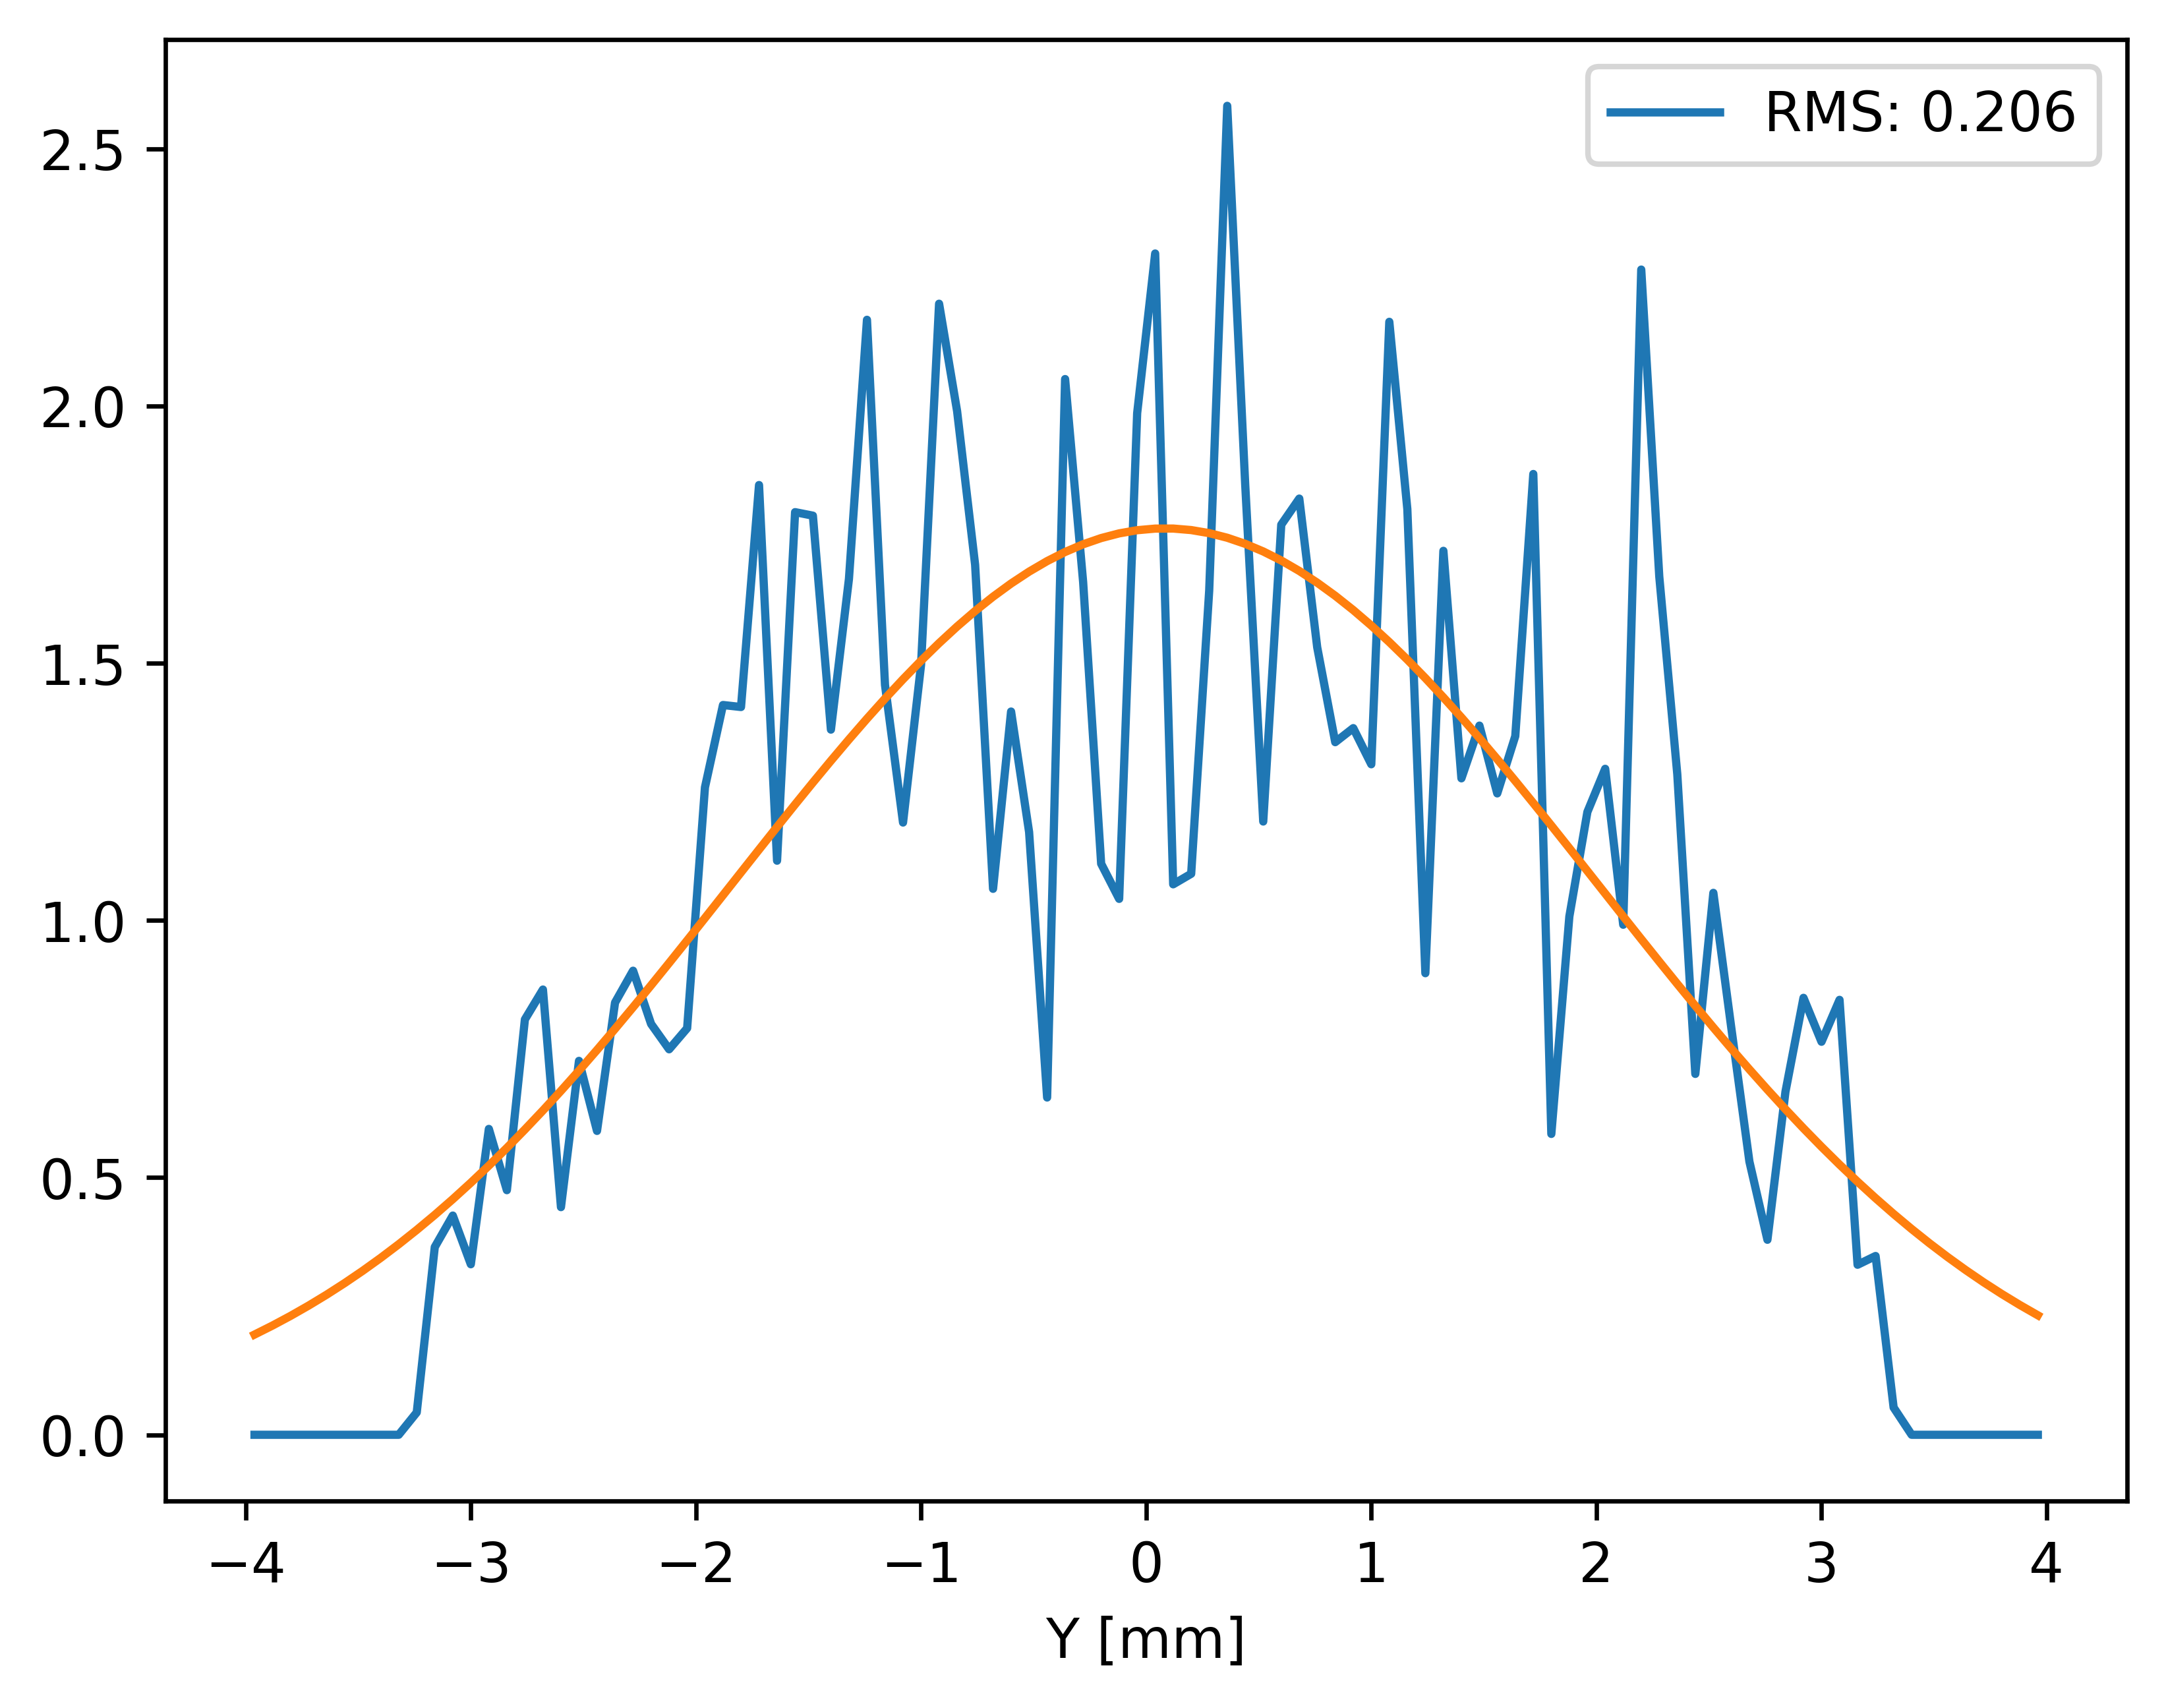
\includegraphics[width=0.9\linewidth]{./../figures/slope_error/WB4C_d30_d-spacing_gradient_45keV_slope_error05urad_Yprofile.png}
\caption{0.5 urad}
\label{fig:05urad}
\end{figure}
